\documentclass[11pt]{article}
\usepackage[T1]{fontenc}
\usepackage{lmodern}
\usepackage{microtype}
\usepackage[a4paper,margin=28mm]{geometry}
\usepackage{amsmath,amssymb,amsthm,mathtools}
\usepackage{booktabs,longtable,array,tabularx}
\usepackage{enumitem}
\usepackage{xcolor}
\usepackage{hyperref}
\usepackage[nameinlink,noabbrev]{cleveref}
\usepackage{listings}
\usepackage{fancyhdr}
\usepackage{lastpage}
\usepackage{graphicx}
\usepackage{url}
\usepackage{tikz}
\usetikzlibrary{arrows.meta,positioning}

\hypersetup{
  colorlinks=true,
  linkcolor=blue!45!black,
  citecolor=green!35!black,
  urlcolor=blue!55!black,
  pdftitle={The normal distribution in intuitionistic primitive recursive arithmetic},
  pdfauthor={OpenAI, prepared for Vladimir Reshetnikov}
}
\pagestyle{fancy}
\fancyhf{}
\lhead{Normal distribution in iPRA}
\rhead{Constructive finite proofs}
\cfoot{\thepage\ of \pageref{LastPage}}
\setlength{\headheight}{14pt}
\setlist{nosep,leftmargin=*}
\setcounter{tocdepth}{2}

\newtheorem{theorem}{Theorem}[section]
\newtheorem{lemma}[theorem]{Lemma}
\newtheorem{proposition}[theorem]{Proposition}
\newtheorem{corollary}[theorem]{Corollary}
\newtheorem{definition}[theorem]{Definition}
\newtheorem{remark}[theorem]{Remark}
\newtheorem{contract}[theorem]{Finite contract}
\newtheorem{algorithm}[theorem]{Algorithm}

\newcommand{\N}{\mathbb N}
\newcommand{\Z}{\mathbb Z}
\newcommand{\Q}{\mathbb Q}
\newcommand{\R}{\mathbb R}
\newcommand{\E}{\mathbb E}
\newcommand{\Pp}{\mathbb P}
\newcommand{\Var}{\operatorname{Var}}
\newcommand{\Cov}{\operatorname{Cov}}
\newcommand{\KL}{D_{\mathrm{KL}}}
\newcommand{\He}{\operatorname{He}}
\newcommand{\erf}{\operatorname{erf}}
\newcommand{\sgn}{\operatorname{sgn}}
\newcommand{\dd}{\,\mathrm d}
\newcommand{\ipra}{\ensuremath{\mathrm{iPRA}}}
\newcommand{\code}[1]{\texttt{\detokenize{#1}}}
\newcommand{\commitsha}{\texttt{8f028dcb4be7a7397d0c11d7c467aa1}\allowbreak\texttt{170cbf2f3}}
\newcommand{\statusP}{\textbf{P}}
\newcommand{\statusE}{\textbf{E}}
\newcommand{\statusR}{\textbf{R}}
\newcommand{\statusC}{\textbf{C}}
\newcommand{\statusD}{\textbf{D}}

\lstset{
  basicstyle=\ttfamily\small,
  breaklines=true,
  frame=single,
  columns=fullflexible,
  showstringspaces=false
}

\title{\textbf{The normal distribution in intuitionistic primitive recursive arithmetic}\\[2mm]
\large A constructive, quantitative reconstruction of the Wikipedia and MathWorld formula collections}
\author{OpenAI\\Prepared for Vladimir Reshetnikov}
\date{16 November 2026}

\begin{document}
\maketitle

\begin{abstract}
We reconstruct a large part of the elementary and intermediate theory of the normal distribution in intuitionistic primitive recursive arithmetic (\ipra).  Since first-order arithmetic has neither a completed real line nor a sort of arbitrary probability measures, every real number, function, integral, and probability law is replaced by a fixed primitive-recursive rational approximation procedure together with explicit error, tail, positivity, or regularity certificates.  Every limiting assertion is expanded into a bounded rational inequality with a primitive-recursive modulus.

Within that discipline we prove normalization, standardization, the density and cumulative-distribution formulas, symmetry, unimodality and inflection points, two global CDF series with remainder bounds, Mills inequalities and a full finite tail expansion, certified values for the $68$--$95$--$99.7$ rule, effective quantiles and safeguarded Newton iteration, all integer moments and the general absolute-moment formula, Hermite derivative identities, conditional moments, Fourier and moment-generating transforms, cumulants, Stein's identity, entropy, Kullback--Leibler and Hellinger formulas, maximum entropy, Fisher information, affine and convolution closure, stability and infinite divisibility, multivariate projection and independence criteria, product, ratio, radial and chi-square laws, exact sampling identities, maximum likelihood, sample-mean and sample-variance theory, and the usual confidence pivots.  The existing ProveIt central-limit packet is used for quantitative CLT claims rather than reproved.

The package includes a statement-by-statement ledger, exact-rational executable certificates (96 checks), a detailed Lean module plan, and explicit target shapes for derivations in ProveIt's deeply embedded \code{Prf PRAAx}.  The Lean files are blueprints, not a claim of a completed kernel-checked analytic development.
\end{abstract}

\tableofcontents
\newpage

\section{Scope, logical meaning, and trust boundary}

\subsection{What ``the normal distribution in \ipra'' can mean}

The ordinary sentence ``let $X$ be a normally distributed real random variable'' quantifies over a completed real line, a sigma-algebra, and a countably additive measure.  None of these is a primitive object of first-order primitive recursive arithmetic.  It would therefore be misleading merely to copy a classical real-analysis proof and announce that it is formalizable.  The correct arithmetical content is a family of finite contracts.

A \emph{fast rational name} is a primitive-recursive map $a\colon\N\to\Q$ satisfying
\begin{equation}\label{eq:fast-name}
  |a(p)-a(q)|\le 2^{-p}+2^{-q}.
\end{equation}
A represented real is not a new object inside the theory: it is convenient metanotation for a fixed program $a$ and the bounded equations asserting \eqref{eq:fast-name} through every requested finite horizon.  An equality $x=y$ means
\[
  \forall p\; |a_x(p+2)-a_y(p+2)|\le 2^{-p},
\]
and an inequality $x\le y$ means the corresponding family of rational inequalities with an explicit tolerance.  Strict positivity is always supplied quantitatively, for example by a witness $r$ with $x\ge 2^{-r}$.  This last point is essential for division by a standard deviation or by a density lower bound.

A function on a bounded rational interval is represented by a primitive-recursive evaluator $F(x,p)$ and a modulus that tells how much input and evaluation precision suffice for an output error $2^{-p}$.  An improper integral is represented by finite quadrature on $[-T,T]$, a mesh-error certificate, and a tail bound beyond $T$.  A probability law is represented either by a finite rational law or by a density/CDF evaluator with these explicit contracts.  Every theorem below is consequently a first-order schema in the codes of the fixed evaluators and certificates.

\begin{remark}[No hidden second-order quantification]
We never postulate a universal evaluator for all primitive-recursive programs and never quantify over ``all real functions'' inside \ipra.  A displayed theorem with parameters such as $f$, $\mu$, or $\sigma$ abbreviates the theorem generated after their concrete primitive-recursive names have been fixed.  Uniform families are allowed when the entire family of evaluators and moduli is itself one primitive-recursive program.
\end{remark}

\subsection{The ambient theory}

The repository's ordinary presentation of \ipra{} has intuitionistic first-order logic with equality, a symbol for every primitive-recursive function together with its defining equations, the successor axioms, and induction for quantifier-free formulas.  In the Lean library the relevant interfaces are the syntax \code{PR} and \code{PTm}, the axiom set \code{PRAAx}, the derivability relation \code{Prf}, and the derived induction rule \code{PRA.qfInd}.  The theorem \code{pra_iff_native} transports completed ordinary derivations to the concise native calculus.  Thus the final formal endpoint for a closed theorem $A$ is not an ambient theorem about \code{Real}; it is a term of type
\[
  []\;\vdash[\code{PRAAx}]\; A,
\]
followed, when desired, by transport through \code{pra\_iff\_native}.

The manuscript supplies human proofs in a deliberately finitary form, identifies every required primitive-recursive operation, gives bounded induction invariants, and lists the target formulas.  It does \emph{not} claim that the analytic collection has already been entered as kernel-checked \code{Prf PRAAx} terms.  The executable Python certificate file is likewise evidence about concrete finite calculations, not a proof oracle for universal statements.

\subsection{Four levels of coverage}

The ledger uses the following labels.
\begin{center}
\begin{tabularx}{0.94\textwidth}{>{\bfseries}l X}
\toprule
P & A complete constructive proof is given for fixed effective presentations; all limits are accompanied by primitive-recursive bounds.\\
E & The classical wording is replaced by its effective version, with the missing modulus, tail bound, apartness, or integrability hypothesis displayed.\\
R & The result is imported from an identified ProveIt packet whose finite proof architecture is used here.\\
C & The source wording needs a qualification or correction; the corrected theorem is proved.\\
D & The statement is recorded but not reconstructed; the missing deep ingredient is named rather than silently assumed.\\
\bottomrule
\end{tabularx}
\end{center}
The labels concern the mathematical proof in this package.  They are not assertions that the corresponding Lean object derivation has already been compiled.

\subsection{Main result at a glance}

\begin{theorem}[Constructive Gaussian package]\label{thm:master}
Fix fast names $\mu$ and $\sigma$, a witness $\sigma\ge 2^{-s_0}>0$, and the standard primitive-recursive approximation contracts for $\pi$, square root, exponential, logarithm, trigonometric functions, and finite Riemann integration described in \cref{sec:representation}.  Then \ipra{} proves, as uniform finite schemas, all results marked P or E in \cref{sec:coverage}.  In particular it proves:
\begin{enumerate}[label=(\roman*)]
  \item the normalization and all elementary shape properties of
  \[
    f_{\mu,\sigma}(x)=\frac{1}{\sigma\sqrt{2\pi}}
       \exp\!\left(-\frac{(x-\mu)^2}{2\sigma^2}\right);
  \]
  \item effective evaluation of the CDF, tails, and quantiles, with explicit rational remainder bounds;
  \item every integer moment, the rational absolute-moment family, all Hermite derivative identities, and the standard transforms;
  \item the entropy, divergence, Hellinger, Fisher-information, and maximum-entropy formulas under explicit effective-integrability contracts;
  \item affine, convolution, multivariate, ratio, product, radial, chi-square, Student and Fisher consequences, and the finite-sample Gaussian statistics described below.
\end{enumerate}
All proofs use only bounded sums and products, rational inequalities, primitive recursion, and quantifier-free induction after the named analytic contracts have been expanded.
\end{theorem}

\begin{proof}[Proof architecture]
The proof is distributed through the manuscript.  The analytic constants and operations are reduced to finite Taylor sums, bisection, and quadrature in \cref{sec:representation}.  Gaussian normalization follows from the effective gamma identity $\Gamma(1/2)=\sqrt\pi$.  Every density identity is then a finite algebraic identity plus an explicit integral substitution.  Integration by parts is the finite telescoping theorem from the calculus packet with Gaussian tail terms discharged by \cref{thm:mills}.  Infinite series are never used without a displayed next-term or geometric remainder.  Transform and convolution theorems use finite rectangles before tail cutoffs are removed.  Information-theoretic statements use the pointwise convex inequality underlying Gibbs' inequality and an explicit integrability modulus.  Multivariate and sample results reduce to finite-dimensional matrix algebra and orthogonal changes of variables.  Finally \cref{sec:internalization} spells out how the bounded verifiers and their invariants become \code{PR} programs and \code{Prf PRAAx} derivations.
\end{proof}

\subsection{Reuse from ProveIt}

The present packet is intentionally complementary to existing work.
\begin{itemize}
  \item The calculus packet supplies represented differentiation, finite Riemann integration, substitutions, integration by parts, and the effective fundamental theorem of calculus.
  \item The gamma packet supplies a primitive-recursive gamma name, the Euler integral, $\Gamma(1/2)=\sqrt\pi$, beta integrals, and rational absolute-moment evaluation.
  \item The Taylor packet supplies finite Taylor formulas with explicit remainders.
  \item The zeta packet contains a quantitative proof of the Gaussian Fourier transform by tail bounds and a first-order differential equation.
  \item The central-limit packet supplies quantitative Berry--Esseen, Lindeberg, de Moivre--Laplace, and related approximation theorems for finite rational laws.  We cite those results in \cref{sec:statistics} rather than duplicate thirty pages of smoothing estimates.
\end{itemize}
Each reuse is at the level of an explicit finite theorem contract.  No conclusion is obtained merely because a classically equivalent theorem exists in Mathlib or ordinary analysis.

\section{Primitive-recursive analytic infrastructure}\label{sec:representation}

This section records enough numerical detail to make the later proofs genuine arithmetic schemas.  The constants are not black boxes: each is generated by a bounded loop with a rational enclosure.

\subsection{Integers, rationals, dyadics, and intervals}

An integer is coded by a sign bit and a natural magnitude.  A rational is a pair $(a,b)$ with $b>0$; equality and order are cross-multiplied integer relations.  Reduction to lowest terms is optional.  Addition, multiplication, absolute value, integer powers, finite sums and products, and dyadic rounding are primitive recursive.  A rational interval is a pair $[l,u]$ with $l\le u$.  The four-endpoint rules for interval multiplication and the reversed-endpoint rule for positive reciprocals are finite case distinctions.

Given a positive rational $q$ and precision $p$, integer bisection finds $m$ such that
\[
  \frac{m^2}{2^{2p}}\le q<\frac{(m+1)^2}{2^{2p}}.
\]
Hence $[m2^{-p},(m+1)2^{-p}]$ encloses $\sqrt q$.  The loop is bounded by an explicit power of two, and its correctness is quantifier-free induction on the search interval.  The same procedure gives an inverse-square-root name once a positive lower bound is supplied.

\subsection{A certified name for \texorpdfstring{$\pi$}{pi}}

For $0\le z\le1$, the finite identity
\[
  \frac{1}{1+t^2}=\sum_{j=0}^{N-1}(-1)^j t^{2j}
      +(-1)^N\frac{t^{2N}}{1+t^2}
\]
and integration from $0$ to $z$ give
\begin{equation}\label{eq:atan-bound}
 \left|\arctan z-\sum_{j=0}^{N-1}(-1)^j\frac{z^{2j+1}}{2j+1}\right|
 \le \frac{z^{2N+1}}{2N+1}.
\end{equation}
Machin's identity
\begin{equation}\label{eq:machin}
 \pi=16\arctan(1/5)-4\arctan(1/239)
\end{equation}
is an exact tangent-addition calculation over the rationals, with the quadrant fixed by the elementary bounds $3<\pi<4$.  Equations \eqref{eq:atan-bound}--\eqref{eq:machin} therefore produce a primitive-recursive interval $\pi_p$ of width at most $2^{-p}$.  The executable certificate uses 170 and 55 terms, then rounds outward to a dyadic interval.  This is far more precision than the displayed numerical table requires.

\subsection{Exponential and logarithm}

For $0\le y\le1$, the alternating sum
\[
 E_N^-(y)=\sum_{j=0}^{N-1}\frac{(-y)^j}{j!}
\]
brackets $e^{-y}$ with its next term:
\begin{equation}\label{eq:exp-alt}
  \min\left(E_N^-(y),E_N^-(y)+\frac{(-y)^N}{N!}\right)
  \le e^{-y}\le
  \max\left(E_N^-(y),E_N^-(y)+\frac{(-y)^N}{N!}\right).
\end{equation}
For $r\ge0$, choose a power of two $m\ge r$, compute an enclosure of $e^{-r/m}$ by \eqref{eq:exp-alt}, and raise the interval to the $m$th power by repeated squaring.  Positive exponentials are reciprocals or use the ordinary positive Taylor sum with the Lagrange remainder.  The computation, its width bound, and monotonicity are all primitive recursive.

For $x>0$, first choose an integer $k$ with $1\le 2^{-k}x<2$, and write
\[
 \log x=k\log2+2\sum_{j=0}^{N-1}
   \frac{u^{2j+1}}{2j+1}+R_N,
 \qquad u=\frac{2^{-k}x-1}{2^{-k}x+1}.
\]
Since $|u|\le1/3$ on $[1,2]$,
\begin{equation}\label{eq:log-tail}
 |R_N|\le \frac{2|u|^{2N+1}}{(2N+1)(1-u^2)}.
\end{equation}
The same series at $x=2$ gives $\log2$.  Thus logarithms on intervals separated from zero have uniform primitive-recursive names.  All later uses of $\log$ state the required positive lower bound.

\subsection{Trigonometric functions}

Range reduction modulo a rational enclosure of $2\pi$, followed by the alternating sine and cosine sums,
\[
 \sin x=\sum_{j<N}\frac{(-1)^j x^{2j+1}}{(2j+1)!}+R_N^{\sin},
 \qquad
 \cos x=\sum_{j<N}\frac{(-1)^j x^{2j}}{(2j)!}+R_N^{\cos},
\]
with the next-term bounds on $|x|\le\pi/4$, gives primitive-recursive trigonometric names.  Exact identities such as $\sin^2x+\cos^2x=1$ are proved first for finite Taylor jets with a controlled remainder or, more economically, by the finite ODE uniqueness theorem from the calculus packet.  Only the Box--Muller section needs these functions.

\subsection{Finite integration contracts}

Let $g$ be represented on $[a,b]$ with an evaluator error $2^{-r}$ and a modulus of uniform continuity $\omega$.  A midpoint mesh with $M$ cells and evaluation precision $r$ produces a rational sum $S_{M,r}$.  Choosing $M$ so that $\omega(M)\le2^{-p-2}/(b-a)$ and $r\ge p+2+\lceil\log_2 M\rceil$ gives
\[
  \left|S_{M,r}-\int_a^b g(x)\dd x\right|\le2^{-p}.
\]
When derivative bounds are available, the midpoint, trapezoidal, or Simpson remainder yields a smaller primitive-recursive mesh.  Improper integrals add a tail producer $T(p)$ satisfying
\[
  \int_{|x|>T(p)} |g(x)|\dd x\le2^{-p}.
\]
All substitutions used below are performed first on finite tagged sums.  The change in mesh and Jacobian is a rational identity; the limit is discharged by the displayed moduli.  This avoids any appeal to a general measure-theoretic change-of-variables theorem inside arithmetic.

\subsection{The gamma input and Gaussian normalization}

The gamma packet provides, for every positive rational $a$ with an apartness witness, a fast name for
\[
 \Gamma(a)=\int_0^\infty t^{a-1}e^{-t}\dd t,
\]
including the functional equation and the certified identity
\begin{equation}\label{eq:gamma-half}
 \Gamma(1/2)=\sqrt\pi.
\end{equation}
For completeness, the Gaussian application is only the positive substitution $t=x^2/2$:
\begin{align*}
 2\int_0^\infty e^{-x^2/2}\dd x
 &=\sqrt2\int_0^\infty t^{-1/2}e^{-t}\dd t\\
 &=\sqrt2\,\Gamma(1/2)=\sqrt{2\pi}.
\end{align*}
Every equality here is an equality of fast rational names.  At a requested precision, truncate both integrals using exponential tails, carry out the substitution on a rational mesh separated from zero, and absorb the small initial interval $[0,\varepsilon]$ by its length bound.  Thus we obtain the normalization contract
\begin{equation}\label{eq:gaussian-normalization}
 \int_{-\infty}^{\infty}\frac{1}{\sqrt{2\pi}}e^{-x^2/2}\dd x=1.
\end{equation}

\subsection{Gaussian tail cutoffs}

The basic tail bound needed to justify every integration by parts is deliberately crude and elementary.  For $T\ge1$ and integer $m\ge0$,
\begin{equation}\label{eq:poly-gaussian-tail}
 \int_T^\infty x^m e^{-x^2/2}\dd x
 \le 2^{m+1}m!\,e^{-T/4}.
\end{equation}
Indeed $x^2/2\ge x/4$ for $x\ge1$, while $x^m\le 2^m m!e^{x/8}$, so the integrand is bounded by $2^m m!e^{-x/8}$ after harmlessly weakening constants.  Integrating the geometric/exponential majorant gives a primitive-recursive cutoff.  Later Mills inequalities provide much sharper bounds, but \eqref{eq:poly-gaussian-tail} already legitimizes polynomially weighted boundary terms.

\begin{contract}[Analytic basis used later]\label{con:analytic-basis}
For every finite precision request and every bounded rational parameter box with the displayed apartness witnesses, there are primitive-recursive procedures returning rational intervals for $\pi$, square roots, exponentials, logarithms, trigonometric functions, Gaussian densities, bounded integrals, and Gaussian improper integrals.  Their correctness predicates are bounded equations and inequalities.  Their composition laws are proved by quantifier-free induction on the finite loops and precision budgets.
\end{contract}

\section{The Gaussian density, CDF, and elementary geometry}\label{sec:gaussian-core}

\subsection{Definitions and standardization}

Define
\begin{equation}\label{eq:phi-def}
 \phi(x)=\frac{1}{\sqrt{2\pi}}e^{-x^2/2},
 \qquad
 \Phi(x)=\int_{-\infty}^{x}\phi(t)\dd t.
\end{equation}
For a location name $\mu$ and a scale name $\sigma$ with $\sigma\ge2^{-s_0}>0$, define
\begin{equation}\label{eq:normal-density}
 f_{\mu,\sigma}(x)=\frac1\sigma\phi\!\left(\frac{x-\mu}{\sigma}\right),
 \qquad
 F_{\mu,\sigma}(x)=\Phi\!\left(\frac{x-\mu}{\sigma}\right).
\end{equation}
The notation $X\sim N(\mu,\sigma^2)$ means that finite interval probabilities are evaluated by $F_{\mu,\sigma}(b)-F_{\mu,\sigma}(a)$, with the represented-integral contract of \cref{sec:representation}.

\begin{theorem}[Normalization and affine standardization]\label{thm:normalization-standardization}
The function $f_{\mu,\sigma}$ is positive and has total integral one.  If $X\sim N(\mu,\sigma^2)$ and $a\ne0$, $b$ are effectively represented, then
\[
 aX+b\sim N(a\mu+b,a^2\sigma^2).
\]
In particular $Z=(X-\mu)/\sigma\sim N(0,1)$.
\end{theorem}

\begin{proof}
Positivity follows from positivity of the exponential, the positive square-root enclosure, and the scale apartness witness.  On a finite interval substitute $z=(x-\mu)/\sigma$ in the tagged Riemann sum; the factor $\sigma$ from the mesh cancels the prefactor $1/\sigma$.  Tail cutoffs transform by the same affine formula.  Equation \eqref{eq:gaussian-normalization} then gives total mass one.

For $Y=aX+b$, interval probabilities satisfy, when $a>0$,
\[
 \Pp(Y\le y)=\Pp\!\left(X\le\frac{y-b}{a}\right)
 =\Phi\!\left(\frac{y-(a\mu+b)}{a\sigma}\right).
\]
When $a<0$ the inequality reverses; symmetry $\Phi(-u)=1-\Phi(u)$, proved below, converts the result to the same formula with scale $|a|\sigma$.  Every comparison is a bounded rational comparison after the finite CDF enclosure is expanded.
\end{proof}

\begin{corollary}[CDF and error-function formulas]\label{cor:cdf-erf}
For all represented $x$,
\begin{align}
 \Phi(x)&=\frac12+\int_0^x\phi(t)\dd t
      =\frac12\left(1+\erf\!\left(\frac{x}{\sqrt2}\right)\right),\label{eq:cdf-erf}\\
 F_{\mu,\sigma}(x)&=\frac12\left(1+\erf\!\left(\frac{x-\mu}{\sigma\sqrt2}\right)\right),
\end{align}
where
\[
 \erf(u)=\frac2{\sqrt\pi}\int_0^u e^{-t^2}\dd t.
\]
\end{corollary}

\begin{proof}
The density is even, so its mass on each half-line is $1/2$.  In the integral from $0$ to $x$, substitute $t=\sqrt2u$ and use $\sqrt2/\sqrt{2\pi}=1/\sqrt\pi$.  This is an equality of finite quadrature names with transformed moduli.
\end{proof}

\subsection{Symmetry, location, and spread}

\begin{theorem}[Symmetry and the three centers]\label{thm:centers}
The standard density is even and the standard CDF satisfies
\begin{equation}\label{eq:cdf-symmetry}
 \Phi(-x)=1-\Phi(x).
\end{equation}
For $N(\mu,\sigma^2)$ the mean, median, and unique mode are all $\mu$.  The variance is $\sigma^2$.
\end{theorem}

\begin{proof}
Evenness is the polynomial identity $(-x)^2=x^2$.  Split the normalized integral at zero and substitute $t\mapsto-t$ on a finite symmetric mesh to obtain \eqref{eq:cdf-symmetry}.  Hence $F_{\mu,\sigma}(\mu)=1/2$, and strict positivity of the density makes the CDF strictly increasing, so the median is unique.

For the standard mean, oddness of $x\phi(x)$ gives cancellation on $[-T,T]$, while \eqref{eq:poly-gaussian-tail} makes the two tails tend effectively to zero.  Thus $\E Z=0$.  Since $\phi'(x)=-x\phi(x)$,
\[
 \E Z^2=\int_{-\infty}^{\infty}x^2\phi(x)\dd x
 =-\int x\phi'(x)\dd x
 =\int\phi(x)\dd x=1,
\]
where the finite integration-by-parts boundary $x\phi(x)|_{-T}^T$ is bounded effectively by \eqref{eq:poly-gaussian-tail}.  Affine standardization gives $\E X=\mu$ and $\Var X=\sigma^2$.

Finally $f'_{\mu,\sigma}(x)=-(x-\mu)f_{\mu,\sigma}(x)/\sigma^2$.  The derivative is positive to the left of $\mu$, zero at $\mu$, and negative to the right.  Rational separation from $\mu$ supplies the strict sign; at an unresolved equality the claim is the non-strict bounded inequality.  Thus the mode is unique.
\end{proof}

\begin{corollary}[Mean absolute deviation, median absolute deviation, skewness and kurtosis]\label{cor:shape-statistics}
For $X\sim N(\mu,\sigma^2)$,
\begin{align*}
 \E|X-\mu|&=\sigma\sqrt{\frac2\pi},\\
 \operatorname{MAD}(X)&=\sigma\Phi^{-1}(3/4),\\
 \operatorname{skew}(X)&=0,\\
 \operatorname{kurt}(X)&=3,
 \qquad \operatorname{excess}(X)=0.
\end{align*}
\end{corollary}

\begin{proof}
For the first identity,
\[
 \E|Z|=2\int_0^\infty x\phi(x)\dd x
 =2\phi(0)=\sqrt{2/\pi},
\]
because $\phi'=-x\phi$.  The median absolute deviation $m$ solves
$\Pp(|X-\mu|\le m)=2\Phi(m/\sigma)-1=1/2$, hence $m/\sigma=\Phi^{-1}(3/4)$.  The third centered moment vanishes by oddness.  The fourth is $3$ by the moment recurrence in \cref{thm:moment-recurrence}, so the standardized kurtosis is $3$.
\end{proof}

\subsection{Differential equations, shape, and log-concavity}

\begin{proposition}[Density and CDF differential equations]\label{prop:gaussian-odes}
The standard density and CDF satisfy
\begin{align}
 \phi'(x)+x\phi(x)&=0, & \phi(0)&=(2\pi)^{-1/2},\label{eq:phi-ode}\\
 \Phi''(x)+x\Phi'(x)&=0, & \Phi(0)&=1/2,
 &\Phi'(0)&=(2\pi)^{-1/2}.
\end{align}
On every bounded interval these initial-value contracts uniquely determine their represented solutions.
\end{proposition}

\begin{proof}
Differentiate the finite exponential approximation and pass its explicit remainder through the product and chain rules.  Since $\Phi'=\phi$ by the effective fundamental theorem of calculus, the second equation follows.  If $u$ and $v$ solve \eqref{eq:phi-ode} with the same initial value, then
\[
 \frac{\dd}{\dd x}\left(e^{x^2/2}(u-v)\right)=0.
\]
The finite fundamental theorem on the segment from $0$ to $x$ makes the product constant, hence zero.  The proof is quantitative: an approximate ODE with residual $\varepsilon$ yields a sup-norm error bounded by the segment length times an explicit exponential factor.
\end{proof}

\begin{proposition}[Peak, inflection points, and log-concavity]\label{prop:shape}
For the standard normal,
\[
 \phi'(x)=-x\phi(x),\qquad \phi''(x)=(x^2-1)\phi(x).
\]
Thus the peak is $\phi(0)=1/\sqrt{2\pi}$, the inflection points are exactly $x=\pm1$, and $\phi$ is strictly log-concave.  For $N(\mu,\sigma^2)$ the peak is $1/(\sigma\sqrt{2\pi})$ and the inflection points are $\mu\pm\sigma$.
\end{proposition}

\begin{proof}
The derivative identities are finite applications of the product and chain rules.  Positivity of $\phi$ reduces the sign of $\phi''$ to the rationally decidable sign of $x^2-1$ away from equality.  Moreover
\[
 \frac{\dd^2}{\dd x^2}\log f_{\mu,\sigma}(x)=-\frac1{\sigma^2}<0.
\]
The logarithm is permitted because the density has a positive lower bound on every bounded parameter box.  The affine formulas follow by the chain rule.
\end{proof}

\begin{corollary}[Strict monotonicity and support]\label{cor:support}
The CDF is strictly increasing, with effective limits $\Phi(x)\to0$ as $x\to-\infty$ and $\Phi(x)\to1$ as $x\to+\infty$.  Every nonempty rational interval has positive Gaussian probability.  Hence the topological support is all of $\R$ in the represented sense: every rational neighborhood receives a computably positive lower bound.
\end{corollary}

\begin{proof}
On $[a,b]$ the density has a computable positive minimum, so
$\Phi(b)-\Phi(a)\ge(b-a)\min_{[a,b]}\phi>0$.  The tail limits follow from \eqref{eq:poly-gaussian-tail}, and later from the sharper Mills bounds.
\end{proof}

\section{CDF series, tails, coverage probabilities, and quantiles}\label{sec:cdf-tails}

\subsection{The ordinary Taylor series with a finite remainder}

Expanding $e^{-t^2/2}$ and integrating term by term only after fixing a finite cutoff gives the safest constructive CDF formula.

\begin{theorem}[Alternating CDF Taylor formula]\label{thm:cdf-taylor}
For every integer $N\ge1$ and represented $x$,
\begin{equation}\label{eq:cdf-taylor}
 \Phi(x)=\frac12+\frac1{\sqrt{2\pi}}
  \sum_{k=0}^{N-1}\frac{(-1)^k x^{2k+1}}{2^k k!(2k+1)}+R_N(x),
\end{equation}
where
\begin{equation}\label{eq:cdf-taylor-rem}
 |R_N(x)|\le
 \frac1{\sqrt{2\pi}}
 \frac{|x|^{2N+1}}{2^N N!(2N+1)}e^{x^2/2}.
\end{equation}
If $N>x^2/2$, the absolute terms decrease from index $N$ onward and the sharper alternating next-term enclosure is valid.
\end{theorem}

\begin{proof}
Taylor's theorem for $e^{-u}$ at $u=0$ gives a finite polynomial plus a Lagrange remainder bounded by $e^{|u|}|u|^N/N!$.  Set $u=t^2/2$, integrate from $0$ to $x$, and bound $|t|\le|x|$.  This yields \eqref{eq:cdf-taylor-rem}.  The ratio of successive integrated term magnitudes is
\[
 \frac{x^2(2k+1)}{2(k+1)(2k+3)}<\frac{x^2}{2(k+1)}.
\]
Thus after $k+1>x^2/2$ the alternating-series theorem applies.  Its proof is the finite pairing inequality for even and odd partial sums, followed by the explicit vanishing of the next term; no countable completeness is used.
\end{proof}

\subsection{A second global series}

The Wikipedia page displays another useful identity, sometimes described there as asymptotic.  It is in fact a convergent equality for every finite $x$.

\begin{theorem}[Convergent density-factor series]\label{thm:cdf-density-series}
For every represented $x$,
\begin{equation}\label{eq:cdf-density-series}
 \Phi(x)=\frac12+\phi(x)
   \sum_{k=0}^{\infty}\frac{x^{2k+1}}{(2k+1)!!}.
\end{equation}
For the $N$-term sum $S_N(x)$,
\begin{equation}\label{eq:density-series-rem}
 \left|\Phi(x)-\frac12-\phi(x)S_N(x)\right|
 \le \frac{\phi(0)|x|^{2N+1}}{(2N-1)!!(2N+1)}.
\end{equation}
Consequently \eqref{eq:cdf-density-series} has a primitive-recursive convergence modulus on every bounded interval.
\end{theorem}

\begin{proof}
Set
\[
 S_N(x)=\sum_{k=0}^{N-1}\frac{x^{2k+1}}{(2k+1)!!}.
\]
Direct coefficient cancellation gives
\[
 S_N'(x)-xS_N(x)=1-\frac{x^{2N}}{(2N-1)!!}.
\]
Using $\phi'=-x\phi$,
\[
 \frac{\dd}{\dd x}(\phi S_N)
 =\phi\left(1-\frac{x^{2N}}{(2N-1)!!}\right).
\]
Subtract from $\Phi'=\phi$, integrate from $0$ to $x$, and use $\Phi(0)=1/2$ and $S_N(0)=0$.  The remainder is
\[
 \frac1{(2N-1)!!}\int_0^x \phi(t)t^{2N}\dd t,
\]
whose absolute value is bounded by \eqref{eq:density-series-rem}.  The ratio of successive majorants tends to zero and is eventually at most $1/2$ with an explicit cutoff $N>|x|^2$, giving the required modulus.
\end{proof}

\begin{remark}[Correction of terminology]
The finite truncations of \eqref{eq:cdf-density-series} can be poor at large $|x|$, because the prefactor is tiny and the positive polynomial sum is large.  That numerical conditioning does not make the series merely asymptotic.  Its tail tends effectively to zero for each bounded $x$, as \eqref{eq:density-series-rem} proves.
\end{remark}

\subsection{Mills inequalities and the complete finite tail expansion}

Write $Q(x)=1-\Phi(x)=\int_x^\infty\phi(t)\dd t$ for $x\ge0$.

\begin{theorem}[Mills inequalities]\label{thm:mills}
For every $x>0$,
\begin{equation}\label{eq:mills}
 \frac{x}{1+x^2}\phi(x)<Q(x)<\frac{\phi(x)}{x}.
\end{equation}
The inequalities are uniform finite contracts on every rational interval $x\in[\delta,B]$ with $\delta>0$.
\end{theorem}

\begin{proof}
For the upper bound, $t/x>1$ for $t>x$, hence
\[
 Q(x)<\frac1x\int_x^\infty t\phi(t)\dd t=\frac{\phi(x)}x.
\]
For the lower bound define
\[
 h(x)=Q(x)-\frac{x}{1+x^2}\phi(x).
\]
A finite differentiation gives
\[
 h'(x)=-\frac{2\phi(x)}{(1+x^2)^2}<0,
\]
while both terms tend effectively to zero as $x\to\infty$.  Therefore $h(x)>0$: for a finite cutoff $T>x$, $h(x)=h(T)-\int_x^T h'(t)\dd t$, the integral is positive, and the explicit tail bound makes $|h(T)|$ smaller than half of that positive rational lower enclosure.  Alternatively one can integrate the pointwise identity obtained from differentiating $x\phi(x)/(1+x^2)$; both versions are primitive recursive.
\end{proof}

\begin{theorem}[Finite alternating tail expansion]\label{thm:mills-expansion}
Let $m\ge1$ and $x>0$.  Then
\begin{equation}\label{eq:tail-expansion}
 Q(x)=\phi(x)\sum_{j=0}^{m-1}
   \frac{(-1)^j(2j-1)!!}{x^{2j+1}}
   +(-1)^m(2m-1)!!J_m(x),
\end{equation}
where
\[
 J_m(x)=\int_x^\infty\frac{\phi(t)}{t^{2m}}\dd t>0.
\]
Thus consecutive truncations bracket $Q(x)$, and
\begin{equation}\label{eq:tail-expansion-error}
 |R_m(x)|<(2m-1)!!\frac{\phi(x)}{x^{2m+1}}.
\end{equation}
\end{theorem}

\begin{proof}
Put $J_j(x)=\int_x^\infty\phi(t)t^{-2j}\dd t$.  Since $\phi'=-t\phi$, finite integration by parts gives
\[
 J_j(x)=\frac{\phi(x)}{x^{2j+1}}-(2j+1)J_{j+1}(x).
\]
Iterate this identity $m$ times.  Positivity gives the alternating bracket, and the upper Mills argument applied to $J_m$ gives
$J_m(x)<\phi(x)/x^{2m+1}$.
\end{proof}

\subsection{The \texorpdfstring{$68$--$95$--$99.7$}{68--95--99.7} rule and certified values}

\begin{corollary}[Central coverage]\label{cor:coverage}
For $Z\sim N(0,1)$,
\[
 \Pp(|Z|\le n)=2\Phi(n)-1=\erf(n/\sqrt2).
\]
The exact-rational certificate program in this package proves the following outward intervals:
\begin{center}
\begin{tabular}{c c}
\toprule
$n$ & certified value of $\Pp(|Z|\le n)$ (decimal display)\\
\midrule
1 & $0.68268949213708589717\ldots$\\
2 & $0.95449973610364158560\ldots$\\
3 & $0.99730020393673981095\ldots$\\
4 & $0.99993665751633376016\ldots$\\
5 & $0.99999942669685624161\ldots$\\
6 & $0.99999999802682470992\ldots$\\
\bottomrule
\end{tabular}
\end{center}
In particular the familiar rounded rule is $68.27\%$, $95.45\%$, and $99.73\%$ for one, two, and three standard deviations.
\end{corollary}

\begin{proof}
The identity follows from symmetry.  For certification, compute a dyadic enclosure of $(2\pi)^{-1/2}$ from Machin's formula and bisection, evaluate \eqref{eq:cdf-taylor} with 220 terms, and use the next-term enclosure because $220>6^2/2$.  Every endpoint is a rational number recorded in \code{evidence/validation.json}; the decimal strings are only renderings of those endpoints.  The same run independently verifies both inequalities in \eqref{eq:mills} for $x=1,\dots,6$.
\end{proof}

\subsection{Effective inverse CDF}

The notation $\Phi^{-1}(p)$ is legitimate constructively only after an algorithm and an error contract are supplied.

\begin{theorem}[Primitive-recursive quantile name]\label{thm:quantile}
Fix a rational $\delta>0$.  There is a primitive-recursive procedure
\[
 \operatorname{qnorm}(p,k)
\]
which, for rational $p\in[\delta,1-\delta]$, returns a rational interval $I_{p,k}$ of width at most $2^{-k}$ containing the unique $q$ with $\Phi(q)=p$.  The correctness proof is uniform in $p$ and $k$.
\end{theorem}

\begin{proof}
Choose $B$ by bounded search so that the upper Mills bound $\phi(B)/B<\delta/4$.  Then $q\in[-B,B]$.  On this compact interval,
\[
 \phi(x)\ge m:=\phi(B)>0,
\]
where $m$ has a certified rational lower bound.  Maintain a bracket $[a,b]$ known to contain a solution up to the current CDF tolerance.  At midpoint $c$, compute an interval $J$ for $\Phi(c)$ of radius
\[
 \varepsilon\le m2^{-k-4}.
\]
If $J$ lies below $p$, replace $a$ by $c$; if it lies above, replace $b$ by $c$.  If $p\in J$, the mean-value estimate
$|\Phi(c)-p|\ge m|c-q|$ shows $|c-q|\le2^{-k-4}$, so return the interval of radius $2^{-k-3}$ about $c$.  Otherwise ordinary bisection reaches width $2^{-k}$ after a primitive-recursive number of steps.  Notice that equality $\Phi(c)=p$ never has to be decided.
\end{proof}

\begin{corollary}[Quantile symmetry and derivatives]\label{cor:quantile-ode}
For $0<p<1$,
\begin{align}
 q(1-p)&=-q(p), & q(1/2)&=0,\label{eq:q-sym}\\
 q'(p)&=\frac1{\phi(q(p))}=\sqrt{2\pi}\,e^{q(p)^2/2},\label{eq:qprime}\\
 q''(p)&=q(p)\,q'(p)^2.\label{eq:qsecond}
\end{align}
On every closed subinterval $[\delta,1-\delta]$ these are effective derivative contracts with explicit bounds.
\end{corollary}

\begin{proof}
Equation \eqref{eq:q-sym} follows from \eqref{eq:cdf-symmetry} and uniqueness.  Differentiate $\Phi(q(p))=p$ on a compact interval where $\phi(q)$ has a positive lower bound.  This gives \eqref{eq:qprime}; differentiating once more and using $\phi'/\phi=-q$ gives \eqref{eq:qsecond}.  The represented derivative theorem uses finite differences and the supplied moduli, not an unbounded inverse-function principle.
\end{proof}

\begin{algorithm}[Safeguarded Newton quantile iteration]\label{alg:newton}
Maintain the bracket from \cref{thm:quantile}.  Given $x_j$ and interval enclosures for $\Phi(x_j)$ and $\phi(x_j)$, form
\[
 y_j=x_j-\frac{\Phi(x_j)-p}{\phi(x_j)}
\]
with enough guard precision, and replace $x_{j+1}$ by $y_j$ if its whole enclosure lies in the bracket; otherwise use the midpoint.  On $[-B,B]$, $\phi\ge m$ and $|\phi'|\le M$, so once $|x_j-q|\le m/(2M)$,
\[
 |x_{j+1}-q|\le \frac{M}{m}|x_j-q|^2
\]
after the rational evaluation errors are budgeted below half the right-hand side.  The initial bisection therefore gives a primitive-recursive entry time into the quadratic regime.
\end{algorithm}

\section{Moments, Hermite polynomials, and conditional expectations}\label{sec:moments}

\subsection{The moment recurrence}

\begin{theorem}[Standard moment recurrence]\label{thm:moment-recurrence}
Let $m_n=\E Z^n$ for $Z\sim N(0,1)$.  Then
\begin{equation}\label{eq:moment-recurrence}
 m_0=1,\qquad m_1=0,\qquad m_{n+2}=(n+1)m_n.
\end{equation}
Consequently
\begin{equation}\label{eq:standard-moments}
 \E Z^{2r+1}=0,
 \qquad
 \E Z^{2r}=(2r-1)!!=\frac{(2r)!}{2^r r!}.
\end{equation}
The theorem is uniform in the externally variable order $n$ and is proved by quantifier-free induction.
\end{theorem}

\begin{proof}
Odd moments vanish by symmetry, with polynomially weighted tails controlled by \eqref{eq:poly-gaussian-tail}.  For $n\ge0$ use $\phi'=-x\phi$:
\[
 m_{n+2}=-\int_{-\infty}^{\infty}x^{n+1}\phi'(x)\dd x
 =(n+1)\int_{-\infty}^{\infty}x^n\phi(x)\dd x.
\]
At a finite cutoff $T$, integration by parts is an exact telescoping identity plus the boundary $T^{n+1}\phi(T)$ at each end.  The primitive-recursive tail schedule chooses $T$ large enough to make the boundary and both omitted integrals smaller than the requested error.  The recurrence is then an equality of names.  Iteration of the recurrence is primitive recursion on $r$ and gives \eqref{eq:standard-moments}.
\end{proof}

\begin{corollary}[Raw moments of a general normal]\label{cor:raw-moments}
For $X\sim N(\mu,\sigma^2)$ and $n\ge0$,
\begin{equation}\label{eq:raw-moment}
 \E X^n=\sum_{j=0}^{\lfloor n/2\rfloor}
  \binom{n}{2j}(2j-1)!!\,\sigma^{2j}\mu^{n-2j}
 =\sum_{j=0}^{\lfloor n/2\rfloor}
  \frac{n!}{2^j j!(n-2j)!}\sigma^{2j}\mu^{n-2j}.
\end{equation}
Equivalently the raw moments obey
\begin{equation}\label{eq:raw-rec}
 M_{n+1}=\mu M_n+n\sigma^2M_{n-1}\qquad(n\ge1).
\end{equation}
\end{corollary}

\begin{proof}
Write $X=\mu+\sigma Z$, expand by the finite binomial theorem, discard odd moments, and insert \eqref{eq:standard-moments}.  Equation \eqref{eq:raw-rec} follows either by coefficient cancellation or by applying Stein's identity to $g(x)=x^n$ after \cref{thm:stein}.  The direct coefficient proof is a finite ring identity and is the preferred object-language route.
\end{proof}

\subsection{Absolute moments}

\begin{theorem}[Absolute moments]\label{thm:absolute-moments}
For every fixed positive rational $p$ (indeed every effectively represented $p>-1$ with the gamma contracts),
\begin{equation}\label{eq:absolute-moment}
 \E|Z|^p=\frac{2^{p/2}\Gamma((p+1)/2)}{\sqrt\pi}.
\end{equation}
Hence
\[
 \E|X-\mu|^p=\sigma^p\frac{2^{p/2}\Gamma((p+1)/2)}{\sqrt\pi}.
\]
For integer $p$, this specializes to the double-factorial formulas above and to
\[
 \E|Z|^{2r+1}=\frac{2^{r+1/2}r!}{\sqrt\pi}.
\]
\end{theorem}

\begin{proof}
By symmetry and the substitution $u=x^2/2$,
\begin{align*}
 \E|Z|^p
 &=\frac2{\sqrt{2\pi}}\int_0^\infty x^p e^{-x^2/2}\dd x\\
 &=\frac{2^{p/2}}{\sqrt\pi}\int_0^\infty
      u^{(p-1)/2}e^{-u}\dd u.
\end{align*}
The last integral is $\Gamma((p+1)/2)$.  Constructively, truncate away from both $0$ and $\infty$, perform the positive substitution on finite meshes, use the gamma packet's near-zero and tail bounds, and then allocate the error budget.  The condition $p>-1$ is exactly what makes the near-zero power integrable and gives a primitive-recursive cutoff once an apartness witness from $-1$ is supplied.
\end{proof}

\subsection{Hermite polynomials and all derivatives}

Define the probabilists' Hermite polynomials by
\begin{equation}\label{eq:hermite-def}
 \He_0(x)=1,
 \quad \He_1(x)=x,
 \quad \He_{n+1}(x)=x\He_n(x)-n\He_{n-1}(x).
\end{equation}
This is a primitive-recursive coefficient array.  Polynomial evaluation and coefficient comparison are bounded folds.

\begin{theorem}[Gaussian derivatives]\label{thm:hermite-derivatives}
For every $n\ge0$,
\begin{align}
 \phi^{(n)}(x)&=(-1)^n\He_n(x)\phi(x),\label{eq:phi-hermite}\\
 f_{\mu,\sigma}^{(n)}(x)&=\frac{(-1)^n}{\sigma^{n+1}}
   \He_n\!\left(\frac{x-\mu}{\sigma}\right)
   \phi\!\left(\frac{x-\mu}{\sigma}\right).
\end{align}
Moreover
\begin{equation}\label{eq:hermite-derivative}
 \He_n'(x)=n\He_{n-1}(x),
\end{equation}
and Rodrigues' formula holds:
\begin{equation}\label{eq:rodrigues}
 \He_n(x)=(-1)^ne^{x^2/2}\frac{\dd^n}{\dd x^n}e^{-x^2/2}.
\end{equation}
\end{theorem}

\begin{proof}
The case $n=0$ is immediate.  If \eqref{eq:phi-hermite} holds at $n$, differentiation gives
\[
 \phi^{(n+1)}=(-1)^n(\He_n'-x\He_n)\phi.
\]
A simultaneous induction proves $\He_n'=n\He_{n-1}$ from \eqref{eq:hermite-def}; substituting it shows the polynomial in parentheses is $-\He_{n+1}$.  This is quantifier-free induction on coefficient lists.  Scaling gives the location-scale formula, and rearranging \eqref{eq:phi-hermite} gives Rodrigues' formula.  The certificate program independently checks the coefficient identity through order 14.
\end{proof}

\begin{corollary}[Hermite orthogonality and norms]\label{cor:hermite-orthogonality}
For integers $m,n\ge0$,
\begin{equation}\label{eq:hermite-orthogonality}
 \int_{-\infty}^{\infty}\He_m(x)\He_n(x)\phi(x)\dd x
 =n!\,\mathbf 1_{m=n}.
\end{equation}
\end{corollary}

\begin{proof}
Assume $m\le n$.  Replace $\He_n\phi$ by $(-1)^n\phi^{(n)}$ and integrate by parts $m$ times.  All boundary terms vanish by the polynomial Gaussian tail bound.  If $m<n$, the $m$th derivative of the degree-$m$ polynomial $\He_m$ is constant and at least one derivative remains on $\phi$; its integral is a vanishing boundary.  If $m=n$, the $n$th derivative of the monic polynomial $\He_n$ is $n!$, leaving $n!\int\phi=n!$.  Every number of integrations is finite and externally indexed, so the proof is a uniform primitive-recursive family.
\end{proof}

\begin{corollary}[Generating function, coefficientwise form]\label{cor:hermite-generating}
For every cutoff $N$,
\begin{equation}\label{eq:hermite-generating}
 e^{tx-t^2/2}=\sum_{n=0}^{N-1}\He_n(x)\frac{t^n}{n!}+R_N(x,t),
\end{equation}
with a primitive-recursive Taylor remainder on each bounded $(x,t)$ box.  Therefore the familiar formal identity
\[
 e^{tx-t^2/2}=\sum_{n\ge0}\He_n(x)t^n/n!
\]
holds as a represented analytic equality.
\end{corollary}

\begin{proof}
Differentiate $e^{tx-t^2/2}$ finitely in $t$.  At $t=0$, the coefficient recurrence is exactly \eqref{eq:hermite-def}.  Taylor's theorem with the bounded exponential remainder proves \eqref{eq:hermite-generating}.  The object theory need only compare the finite coefficient arrays and verify the supplied remainder bound.
\end{proof}

\subsection{Truncated and conditional moments}

Let $\alpha=(a-\mu)/\sigma$, $\beta=(b-\mu)/\sigma$, and
$Z_{\alpha,\beta}=\Phi(\beta)-\Phi(\alpha)$.  Assume a positive lower bound on this interval probability.

\begin{theorem}[Conditional mean and variance on an interval]\label{thm:truncated-normal}
For $a<b$,
\begin{align}
 \E[X\mid a<X<b]
 &=\mu+\sigma\frac{\phi(\alpha)-\phi(\beta)}{Z_{\alpha,\beta}},\label{eq:trunc-mean}\\
 \Var(X\mid a<X<b)
 &=\sigma^2\left[
 1+\frac{\alpha\phi(\alpha)-\beta\phi(\beta)}{Z_{\alpha,\beta}}
 -\left(\frac{\phi(\alpha)-\phi(\beta)}{Z_{\alpha,\beta}}\right)^2
 \right].\label{eq:trunc-var}
\end{align}
One-sided truncations follow by sending an endpoint to infinity with the Mills modulus.
\end{theorem}

\begin{proof}
Standardize.  Since $z\phi(z)=-\phi'(z)$,
\[
 \int_\alpha^\beta z\phi(z)\dd z=\phi(\alpha)-\phi(\beta).
\]
Also integration by parts gives
\[
 \int_\alpha^\beta z^2\phi(z)\dd z
 =Z_{\alpha,\beta}+\alpha\phi(\alpha)-\beta\phi(\beta).
\]
Divide by the positive interval mass, transform back to $X=\mu+\sigma Z$, and subtract the square of the mean.  The denominator's lower bound is computable from the positive minimum of the density on $[\alpha,\beta]$.
\end{proof}

\begin{proposition}[Recursive incomplete moments]\label{prop:incomplete-moments}
For $I_n(a,b)=\int_a^b x^n\phi(x)\dd x$,
\begin{equation}\label{eq:incomplete-rec}
 I_n(a,b)=\bigl[-x^{n-1}\phi(x)\bigr]_a^b+(n-1)I_{n-2}(a,b)
 \qquad(n\ge2).
\end{equation}
Thus every finite truncated integer moment reduces to $\Phi$ and endpoint density values by primitive recursion.
\end{proposition}

\begin{proof}
Use $x\phi=-\phi'$ and integrate $x^{n-1}(-\phi')$ by parts on the bounded interval.  No improper limit occurs.
\end{proof}

\section{Transforms, cumulants, Stein's identity, and effective characterizations}\label{sec:transforms}

\subsection{Moment-generating and characteristic functions}

\begin{theorem}[MGF, characteristic function, and Fourier transform]\label{thm:transforms}
For $X\sim N(\mu,\sigma^2)$ and represented real $t$,
\begin{align}
 M_X(t)&=\E e^{tX}=\exp\!\left(\mu t+\frac12\sigma^2t^2\right),\label{eq:mgf}\\
 \chi_X(t)&=\E e^{itX}=\exp\!\left(i\mu t-\frac12\sigma^2t^2\right).
 \label{eq:cf}
\end{align}
With the Fourier convention $\widehat f(\xi)=\int f(x)e^{-2\pi i\xi x}\dd x$,
\begin{equation}\label{eq:fourier}
 \widehat{f_{\mu,\sigma}}(\xi)
 =e^{-2\pi i\mu\xi}e^{-2\pi^2\sigma^2\xi^2}.
\end{equation}
All three identities are uniform on bounded parameter boxes; the MGF is uniform on every bounded $t$ interval.
\end{theorem}

\begin{proof}
For the MGF, complete the square by an exact polynomial identity:
\[
 tx-\frac{(x-\mu)^2}{2\sigma^2}
 =-\frac{(x-\mu-\sigma^2t)^2}{2\sigma^2}
   +\mu t+\frac12\sigma^2t^2.
\]
Factor out the constant and translate the normalized Gaussian integral.  On a finite interval this is a rational identity between exponential evaluators; the shifted tails are controlled uniformly by \eqref{eq:poly-gaussian-tail}.

For the characteristic function one may repeat the argument with complex rational pairs, but a fully real proof is cleaner.  Let
\[
 C(t)=\int\phi(x)\cos(tx)\dd x,\qquad
 S(t)=\int\phi(x)\sin(tx)\dd x.
\]
Oddness gives $S(t)=0$.  Differentiate the finite integral, use $x\phi=-\phi'$, and integrate by parts to obtain $C'(t)=-tC(t)$ with $C(0)=1$.  The ODE uniqueness argument of \cref{prop:gaussian-odes} gives $C(t)=e^{-t^2/2}$.  Translation and scaling give \eqref{eq:cf}; substituting $t=2\pi\xi$ gives \eqref{eq:fourier}.  This is the same quantitative architecture as the Gaussian transform proved in the ProveIt zeta packet.
\end{proof}

\begin{corollary}[Self-reciprocal Gaussian]\label{cor:self-fourier}
Under the convention of \eqref{eq:fourier}, $x\mapsto e^{-\pi x^2}$ is fixed by the Fourier transform.  More generally
\[
 \int_{-\infty}^{\infty}e^{-\pi a x^2}e^{-2\pi ibx}\dd x
 =a^{-1/2}e^{-\pi b^2/a}
\]
for every positive represented $a$.
\end{corollary}

\begin{proof}
Scale \eqref{eq:fourier}, or solve the same transform ODE with the normalization obtained from \eqref{eq:gaussian-normalization}.  The positive inverse square root uses the supplied apartness witness for $a$.
\end{proof}

\subsection{Cumulants and Wick's formula}

\begin{corollary}[Cumulants]\label{cor:cumulants}
The cumulant-generating function is
\begin{equation}\label{eq:cgf}
 K_X(t)=\log M_X(t)=\mu t+\frac12\sigma^2t^2.
\end{equation}
Hence
\[
 \kappa_1=\mu,\qquad \kappa_2=\sigma^2,
 \qquad \kappa_n=0\quad(n\ge3).
\]
This proves the normal distribution's vanishing higher cumulants.  It does not by itself prove the full Marcinkiewicz characterization of all distributions with only finitely many nonzero cumulants.
\end{corollary}

\begin{proof}
On a bounded $t$ interval $M_X(t)$ has an explicit positive lower bound, so the represented logarithm is defined.  Apply it to \eqref{eq:mgf} and compare finite Taylor coefficients.  Derivatives of a quadratic vanish after order two by exact arithmetic.
\end{proof}

\begin{theorem}[Finite Wick--Isserlis formula]\label{thm:wick}
Let $(X_1,\dots,X_d)$ be a centered jointly Gaussian vector with covariance matrix $\Sigma$.  For every finite index list $i_1,\dots,i_n$,
\[
 \E\prod_{r=1}^nX_{i_r}=0\quad\text{if $n$ is odd},
\]
and for $n=2m$,
\begin{equation}\label{eq:wick}
 \E\prod_{r=1}^{2m}X_{i_r}
 =\sum_{\text{pairings }P}\prod_{\{r,s\}\in P}\Sigma_{i_r i_s}.
\end{equation}
The sum is over the finite primitive-recursively enumerable set of pairings.
\end{theorem}

\begin{proof}
The multivariate MGF is $\exp(\tfrac12 t^T\Sigma t)$.  Fix the finite order $n$, replace the exponential by its Taylor polynomial through degree $n$, and extract the coefficient of $t_{i_1}\cdots t_{i_n}$.  Odd total degree is absent.  In degree $2m$, choosing $m$ quadratic factors is exactly choosing a pairing; the factorials cancel the ordering multiplicities.  This is a finite polynomial identity.  Alternatively, repeated multivariate integration by parts gives the same pairing recurrence.
\end{proof}

\subsection{Stein's identity and characterization}

\begin{theorem}[Stein identity]\label{thm:stein}
Let $X\sim N(\mu,\sigma^2)$.  Suppose $g$ has an effective derivative on every bounded interval and a primitive-recursive growth bound making $g(x)f_{\mu,\sigma}(x)$ vanish at both tails.  Then
\begin{equation}\label{eq:stein}
 \E[(X-\mu)g(X)]=\sigma^2\E[g'(X)].
\end{equation}
\end{theorem}

\begin{proof}
The density derivative satisfies
$f'_{\mu,\sigma}=-(x-\mu)f_{\mu,\sigma}/\sigma^2$.  Therefore on $[-T,T]$,
\[
 \int (x-\mu)g(x)f(x)\dd x
 =-\sigma^2\int g(x)f'(x)\dd x
 =\sigma^2\int g'(x)f(x)\dd x
   -\sigma^2[g(x)f(x)]_{-T}^T.
\]
The growth/tail contract makes the boundary smaller than any requested dyadic error.  The remaining two integrals have the ordinary finite quadrature contracts.
\end{proof}

\begin{theorem}[Effective Stein characterization]\label{thm:stein-characterization}
Let $Y$ be an effectively presented probability law with finite second moment.  Assume that for every represented trigonometric test $g_t(x)=e^{itx}$ on every bounded $t$ interval,
\begin{equation}\label{eq:stein-assumption}
 \E[(Y-\mu)g_t(Y)]=\sigma^2\E[g_t'(Y)]
\end{equation}
holds with a uniform primitive-recursive modulus.  Then the characteristic function of $Y$ equals \eqref{eq:cf}; consequently all finite interval probabilities agree effectively with $N(\mu,\sigma^2)$.
\end{theorem}

\begin{proof}
Let $\chi(t)=\E e^{itY}$.  Equation \eqref{eq:stein-assumption} becomes
\[
 \frac1i\chi'(t)-\mu\chi(t)=i\sigma^2t\chi(t),
\]
after differentiating under the effective second-moment bound.  Thus
$\chi'(t)=(i\mu-\sigma^2t)\chi(t)$ and $\chi(0)=1$.  Multiplying by
$e^{-i\mu t+\sigma^2t^2/2}$ gives a function with zero derivative, hence the normal characteristic function by finite ODE uniqueness.

To pass from characteristic functions to interval probabilities constructively, convolve both laws with the finite triangular smoothing kernel used in the central-limit packet.  Fourier inversion for that compactly supported kernel is a finite integral identity.  Equality of the characteristic functions gives equality of the smoothed CDFs, and the supplied tightness plus anti-concentration modulus lets the smoothing width tend effectively to zero at rational interval endpoints.
\end{proof}

\subsection{What is and is not characterized}

\begin{proposition}[Quadratic log-MGF criterion]\label{prop:quadratic-mgf}
If an effective law has an MGF on a rational neighborhood of zero and its represented logarithm is exactly
$\mu t+\sigma^2t^2/2$ there, then the law is $N(\mu,\sigma^2)$.
\end{proposition}

\begin{proof}
Exponentiate to recover \eqref{eq:mgf}, substitute imaginary arguments through the common finite power series, and apply the characteristic-function uniqueness step above.  Equivalently, equality of all derivatives at zero plus an explicit analytic remainder gives equality of MGFs on a neighborhood and then of characteristic functions.
\end{proof}

\begin{remark}[Deep classical characterizations]
The stronger Marcinkiewicz theorem (a polynomial log characteristic function has degree at most two), Cramer's decomposition theorem, the Kac--Bernstein theorem, and Geary's characterization by independence of sample mean and variance require substantial additional harmonic or functional-equation arguments.  They are listed as D in the ledger.  This package proves every forward Gaussian statement used by those theorems, and the analytic quadratic-MGF criterion, but does not disguise those deeper converses as elementary consequences of cumulant algebra.
\end{remark}

\section{Entropy, divergence, Hellinger distance, Fisher information, and maxima}\label{sec:information}

The formulas in this section involve logarithms of densities or ratios.  The constructive statements therefore include the following standard contract: each density has a fixed primitive-recursive evaluator, the relevant logarithm is requested only where a positive lower bound is known, and the integral has explicit near-zero and tail moduli.  For a Gaussian density these conditions are automatic on bounded intervals and the tails are controlled by \cref{thm:mills}.  For a comparison density in the maximum-entropy theorem they are hypotheses rather than consequences of the word ``density.''

\subsection{Differential entropy}

\begin{theorem}[Gaussian entropy]\label{thm:entropy}
For $X\sim N(\mu,\sigma^2)$,
\begin{equation}\label{eq:entropy}
 h(X)=-\int f_{\mu,\sigma}(x)\log f_{\mu,\sigma}(x)\dd x
 =\frac12\log(2\pi e\sigma^2).
\end{equation}
The value is independent of $\mu$, and $h(aX+b)=h(X)+\log|a|$ for $a\ne0$.
\end{theorem}

\begin{proof}
The exact identity
\[
 -\log f_{\mu,\sigma}(x)
 =\log(\sigma\sqrt{2\pi})+\frac{(x-\mu)^2}{2\sigma^2}
\]
reduces the integral to normalization and variance.  Therefore
\[
 h(X)=\log(\sigma\sqrt{2\pi})+\frac12
 =\frac12\log(2\pi e\sigma^2).
\]
Every term is an effective name.  The affine formula follows either by substitution in the integral or by replacing $\sigma$ with $|a|\sigma$.
\end{proof}

\subsection{Kullback--Leibler divergence}

\begin{theorem}[KL divergence of two normals]\label{thm:kl-normal}
Let $P=N(\mu_0,\sigma_0^2)$ and $Q=N(\mu_1,\sigma_1^2)$, with positive scale witnesses.  Then
\begin{equation}\label{eq:kl-normal}
 \KL(P\Vert Q)
 =\log\frac{\sigma_1}{\sigma_0}
 +\frac{\sigma_0^2+(\mu_0-\mu_1)^2}{2\sigma_1^2}-\frac12.
\end{equation}
It is nonnegative and is zero exactly when $\mu_0=\mu_1$ and $\sigma_0=\sigma_1$ in the represented equality sense.
\end{theorem}

\begin{proof}
Subtract the two log-density formulas and take expectation under $P$.  The only inputs are
$\E_P(X-\mu_0)^2=\sigma_0^2$ and
$\E_P(X-\mu_1)^2=\sigma_0^2+(\mu_0-\mu_1)^2$, giving \eqref{eq:kl-normal}.

For nonnegativity, put $r=\sigma_0^2/\sigma_1^2>0$ and $d=(\mu_0-\mu_1)^2/\sigma_1^2\ge0$.  Twice the divergence is
\[
 r-1-\log r+d.
\]
The scalar inequality $\log r\le r-1$ follows from
\[
 r-1-\log r=\int_1^r\left(1-\frac1t\right)\dd t\ge0,
\]
with the orientation reversed when $r<1$; the integrand has the appropriate sign on the bounded interval.  Equality forces $r=1$ and $d=0$.  The effective strict statement uses an apartness witness; without one, the non-strict inequality is the internal formula.
\end{proof}

\begin{lemma}[Gibbs inequality in finite-contract form]\label{lem:gibbs}
Let $p$ and $q$ be effective densities with $q>0$ and with explicit integrability moduli for $p\log(p/q)$.  Then
\[
 \int p\log\frac pq\dd x\ge0.
\]
\end{lemma}

\begin{proof}
The pointwise inequality $u\log u-u+1\ge0$ for $u\ge0$ follows by calculus on a bounded interval and the convention $0\log0=0$ with its explicit limiting bound.  Set $u=p/q$, multiply by $q$, and integrate:
\[
 p\log(p/q)-p+q\ge0.
\]
Normalization cancels the last two integrals.  Constructively, truncate to a finite interval, replace very small $p$ by the elementary bound $|p\log p|\le C\sqrt p$, and use the supplied tail modulus.  All pointwise comparisons are rational interval comparisons.
\end{proof}

\subsection{Maximum entropy}

\begin{theorem}[Gaussian maximum entropy]\label{thm:max-entropy}
Let $p$ be an effectively presented density with mean $\mu$, variance $\sigma^2>0$, finite entropy, and the integrability contracts required by \cref{lem:gibbs}.  Then
\begin{equation}\label{eq:max-entropy}
 h(p)\le\frac12\log(2\pi e\sigma^2),
\end{equation}
with equality only when $p=f_{\mu,\sigma}$ almost everywhere in the effective $L^1$ sense.
\end{theorem}

\begin{proof}
Let $g=f_{\mu,\sigma}$.  Since $-\log g$ is a constant plus $(x-\mu)^2/(2\sigma^2)$, the matching first two moments give
\[
 -\int p\log g=\frac12\log(2\pi e\sigma^2)=h(g).
\]
Therefore
\[
 \KL(p\Vert g)=\int p\log p-\int p\log g=h(g)-h(p)\ge0
\]
by \cref{lem:gibbs}.  Equality in the pointwise convex inequality forces $p/g=1$ wherever the effective mass is nonzero; quantitatively, the finite Pinsker inequality
$\|p-g\|_1^2\le2\KL(p\Vert g)$ gives the represented $L^1$ conclusion.
\end{proof}

\begin{remark}[The hypothesis is not merely ``has a variance'']
A bare classical density with a finite second moment does not automatically carry a primitive-recursive entropy or KL integrability modulus.  The maximum-entropy theorem is therefore marked E: it is fully proved for effective densities with the displayed contracts, not asserted for an unrepresented totality of all measures.
\end{remark}

\subsection{Hellinger affinity and equal-variance total variation}

\begin{theorem}[Hellinger formula]\label{thm:hellinger}
For the convention
$H^2(P,Q)=1-\int\sqrt{pq}$, two normal laws satisfy
\begin{equation}\label{eq:hellinger}
 H^2(P,Q)=1-
 \sqrt{\frac{2\sigma_0\sigma_1}{\sigma_0^2+\sigma_1^2}}
 \exp\!\left(-\frac{(\mu_0-\mu_1)^2}{4(\sigma_0^2+\sigma_1^2)}\right).
\end{equation}
\end{theorem}

\begin{proof}
Multiply the square roots of the two densities.  Completing the square writes the exponent as a normalized Gaussian with variance
$2\sigma_0^2\sigma_1^2/(\sigma_0^2+\sigma_1^2)$ plus the constant
$-(\mu_0-\mu_1)^2/[4(\sigma_0^2+\sigma_1^2)]$.  Integrate the normalized factor and simplify the rational square roots.  The completion is a finite polynomial identity; positivity of the denominators is supplied by the scale witnesses.
\end{proof}

\begin{proposition}[Total variation for equal scales]\label{prop:tv-equal-scale}
For $P=N(\mu_0,\sigma^2)$ and $Q=N(\mu_1,\sigma^2)$,
\begin{equation}\label{eq:tv-equal-scale}
 \|P-Q\|_{\mathrm{TV}}
 =2\Phi\!\left(\frac{|\mu_0-\mu_1|}{2\sigma}\right)-1.
\end{equation}
\end{proposition}

\begin{proof}
Assume $\mu_1>\mu_0$.  The two densities cross exactly at $c=(\mu_0+\mu_1)/2$, because their log ratio is an affine function of $x$.  Integrating the positive difference on $(c,\infty)$ and standardizing gives
$\Phi((\mu_1-\mu_0)/(2\sigma))-\Phi(-(\mu_1-\mu_0)/(2\sigma))$, which is \eqref{eq:tv-equal-scale}.  The other order follows by symmetry.
\end{proof}

\subsection{Fisher information}

\begin{theorem}[Fisher information matrices]\label{thm:fisher}
For parameters $(\mu,\sigma)$, the score functions are
\[
 S_\mu(X)=\frac{X-\mu}{\sigma^2},
 \qquad
 S_\sigma(X)=-\frac1\sigma+\frac{(X-\mu)^2}{\sigma^3},
\]
and the Fisher information is
\begin{equation}\label{eq:fisher-musigma}
 I(\mu,\sigma)=
 \begin{pmatrix}
  \sigma^{-2}&0\\[1mm]
  0&2\sigma^{-2}
 \end{pmatrix}.
\end{equation}
For parameters $(\mu,v)$ with $v=\sigma^2$,
\begin{equation}\label{eq:fisher-muv}
 I(\mu,v)=
 \begin{pmatrix}
  v^{-1}&0\\[1mm]
  0&(2v^2)^{-1}
 \end{pmatrix}.
\end{equation}
For $n$ independent observations the matrix is multiplied by $n$.
\end{theorem}

\begin{proof}
Differentiate the explicit log density on a bounded parameter box separated from $\sigma=0$.  Standardize $X-\mu=\sigma Z$ and use $\E Z=0$, $\E Z^2=1$, $\E Z^3=0$, $\E Z^4=3$.  This gives
$\E S_\mu^2=1/\sigma^2$, $\E S_\mu S_\sigma=0$, and
$\E S_\sigma^2=(3-2+1)/\sigma^2=2/\sigma^2$.  The $v$ formula follows by the finite chain rule.  Independence makes log likelihoods and scores finite sums, so cross-observation terms vanish by the zero score mean.
\end{proof}

\subsection{Maximum of Gaussian variables}

\begin{theorem}[Expected maximum bound]\label{thm:expected-max}
Let $X_1,\dots,X_n$ be Gaussian random variables with means at most $\mu$ and variances at most $\sigma^2$.  Independence is not required.  Then for $n\ge2$,
\begin{equation}\label{eq:expected-max}
 \E\max_{j\le n}X_j\le \mu+\sigma\sqrt{2\log n}.
\end{equation}
The statement is effective for a finite jointly presented law and fixed $n$.
\end{theorem}

\begin{proof}
For any rational $t>0$,
\[
 e^{t\max_jX_j}\le\sum_{j=1}^ne^{tX_j}.
\]
By concavity of $\log$ in its finite Jensen form,
\[
 t\E\max_jX_j
 \le \log\E e^{t\max_jX_j}
 \le \log\sum_j\E e^{tX_j}
 \le \log n+t\mu+\frac12t^2\sigma^2.
\]
Divide by $t$ and choose $t=\sqrt{2\log n}/\sigma$ when $\sigma>0$.  Square root and logarithm are effective because $n\ge2$.  If $\sigma=0$, every variable is degenerate at its mean and the inequality is immediate.  The finite Jensen inequality follows from the convexity of $e^x$ or the weighted AM--GM inequality with rational approximation; it needs no independence.
\end{proof}

\section{Affine closure, sums, stability, and multivariate normals}\label{sec:closure}

\subsection{Sums and linear combinations}

\begin{theorem}[Independent Gaussian linear combinations]\label{thm:linear-combination}
Let $X_j\sim N(\mu_j,\sigma_j^2)$ be independent for $1\le j\le n$, and let $a_j$ be represented scalars.  Then
\begin{equation}\label{eq:linear-combination}
 \sum_{j=1}^na_jX_j
 \sim N\!\left(\sum_ja_j\mu_j,\ \sum_ja_j^2\sigma_j^2\right).
\end{equation}
In particular, the sum of independent normals is normal.
\end{theorem}

\begin{proof}
Independence of a finite product law is the exact factorization of its rectangular weights or density.  Fubini is first a finite double-sum identity after truncation.  Therefore the characteristic function of the sum is the product of the characteristic functions:
\[
 \prod_j\exp\!\left(ia_j\mu_jt-\frac12a_j^2\sigma_j^2t^2\right)
 =\exp\!\left(it\sum_ja_j\mu_j-\frac12t^2\sum_ja_j^2\sigma_j^2\right).
\]
Apply the effective characteristic-function uniqueness argument of \cref{thm:stein-characterization}.  The entire calculation is a finite sum in the exponent.
\end{proof}

\begin{corollary}[Stability and infinite divisibility]\label{cor:stability}
The normal family is stable.  If $X_1,X_2$ are independent copies of $N(\mu,\sigma^2)$ and $a,b$ are scalars, then
\[
 aX_1+bX_2\sim N((a+b)\mu,(a^2+b^2)\sigma^2).
\]
For every $n\ge1$,
\[
 N(\mu,\sigma^2)
 =\underbrace{N(\mu/n,\sigma^2/n)*\cdots*N(\mu/n,\sigma^2/n)}_{n\text{ factors}},
\]
so the normal law is infinitely divisible in the finite arithmetical sense.
\end{corollary}

\begin{proof}
This is \cref{thm:linear-combination}.  The infinite-divisibility statement has one finite convolution identity for each $n$; no actual infinite convolution is formed.
\end{proof}

\begin{proposition}[Normalized product of Gaussian densities]\label{prop:product-densities}
Let $f_j$ be Gaussian densities $N(\mu_j,\sigma_j^2)$ and let $w_j>0$ be rational weights.  The normalized weighted geometric product
\[
 g(x)=\frac{\prod_j f_j(x)^{w_j}}
 {\int\prod_j f_j(t)^{w_j}\dd t}
\]
is Gaussian with precision and mean
\begin{equation}\label{eq:precision-pool}
 \tau^{-2}=\sum_j\frac{w_j}{\sigma_j^2},
 \qquad
 m=\tau^2\sum_j\frac{w_j\mu_j}{\sigma_j^2}.
\end{equation}
\end{proposition}

\begin{proof}
Take logarithms.  The $x$-dependent part is
$-\tfrac12\sum_jw_j(x-\mu_j)^2/\sigma_j^2$.  Completing the square gives
$-(x-m)^2/(2\tau^2)$ plus a constant.  The positive normalizing integral is then the Gaussian normalization.  All exponents and sums are finite; logarithmic powers are evaluated on positive density intervals.
\end{proof}

\subsection{Multivariate definition and transforms}

Let $\Sigma$ be a symmetric positive-definite $d\times d$ matrix of represented numbers.  Constructively, positive definiteness is accompanied by a rational witness $\lambda>0$ such that
$v^T\Sigma v\ge\lambda\|v\|^2$ for rational vectors in the relevant finite precision.  This yields apartness of $\det\Sigma$, an inverse-matrix name, and stable Cholesky or $LDL^T$ elimination.

\begin{definition}[Multivariate normal]
The law $N_d(\mu,\Sigma)$ has density
\begin{equation}\label{eq:multi-density}
 f(x)=\frac{1}{(2\pi)^{d/2}(\det\Sigma)^{1/2}}
 \exp\!\left(-\frac12(x-\mu)^T\Sigma^{-1}(x-\mu)\right).
\end{equation}
Equivalently, $X=\mu+AZ$ where $Z$ has independent standard-normal coordinates and $AA^T=\Sigma$.
\end{definition}

\begin{theorem}[Multivariate normalization and characteristic function]\label{thm:multivariate-normal}
The density \eqref{eq:multi-density} integrates to one, and
\begin{equation}\label{eq:multi-cf}
 \E e^{it^TX}=\exp\!\left(it^T\mu-\frac12t^T\Sigma t\right).
\end{equation}
Every rational linear image $BX+c$ is
\begin{equation}\label{eq:multi-affine}
 BX+c\sim N_k(B\mu+c,B\Sigma B^T),
\end{equation}
with the natural possibly degenerate interpretation when $B\Sigma B^T$ is singular.
\end{theorem}

\begin{proof}
For a nonsingular rational approximation $A$ to a Cholesky factor, perform the linear substitution $x=\mu+Az$ on a finite box.  Determinants are finite Leibniz sums, and the Jacobian cancellation is an exact matrix identity.  The approximation error is controlled by the matrix perturbation witness and the Gaussian tails.  Equivalently, define the law by the affine image of independent coordinates; normalization is automatic.  Formula \eqref{eq:multi-cf} is the finite product of scalar characteristic functions.  Replacing $t$ by $B^Tt$ proves \eqref{eq:multi-affine}.
\end{proof}

\begin{corollary}[Projections, marginals, and ellipsoids]\label{cor:projections}
For every vector $a$,
\[
 a^TX\sim N(a^T\mu,a^T\Sigma a).
\]
Every coordinate subvector is multivariate normal with the corresponding principal covariance block.  The positive-density level sets are ellipsoids
\[
 (x-\mu)^T\Sigma^{-1}(x-\mu)=c.
\]
Whitening by any effective $A^{-1}$ with $AA^T=\Sigma$ produces a standard spherical normal.
\end{corollary}

\begin{proof}
Projection and marginal statements are instances of \eqref{eq:multi-affine}.  Taking the logarithm of \eqref{eq:multi-density} leaves a constant minus half the displayed quadratic form, so level sets have the stated equation.
\end{proof}

\subsection{Uncorrelated jointly normal variables are independent}

\begin{theorem}[Block independence]\label{thm:joint-normal-independence}
If a jointly Gaussian vector $(U,V)$ has block covariance
\[
 \Sigma=\begin{pmatrix}\Sigma_U&0\\0&\Sigma_V\end{pmatrix},
\]
then $U$ and $V$ are independent.  In particular, jointly normal scalar variables are independent exactly when their covariance is zero, except for the trivial degenerate qualifications.
\end{theorem}

\begin{proof}
The characteristic function factors:
\[
 e^{i(s^T\mu_U+t^T\mu_V)-\frac12(s^T\Sigma_Us+t^T\Sigma_Vt)}
 =\chi_U(s)\chi_V(t).
\]
Apply effective transform uniqueness on finite rectangles.  If both variances are positive, independence implies zero covariance by finite product integration, giving the converse.  Degenerate constants are independent of every law in the usual finite-product sense.
\end{proof}

\begin{corollary}[Sum and difference]\label{cor:sum-difference}
If $X,Y$ are independent $N(\mu,\sigma^2)$ variables, then $X+Y$ and $X-Y$ are independent, with laws $N(2\mu,2\sigma^2)$ and $N(0,2\sigma^2)$.
\end{corollary}

\begin{proof}
The pair is jointly Gaussian.  Its transformed covariance is
$\Cov(X+Y,X-Y)=\Var X-\Var Y=0$.  Apply \cref{thm:joint-normal-independence}.
\end{proof}

\subsection{Conditional multivariate normals}

\begin{theorem}[Bivariate conditional law]\label{thm:bivariate-conditional}
Let $(X,Y)$ be jointly normal with positive scales $\sigma_X,\sigma_Y$ and correlation $|\rho|<1$ with an apartness witness.  At a represented observation $Y=y$, the conditional density of $X$ is
\begin{equation}\label{eq:conditional-normal}
 X\mid(Y=y)\sim N\!\left(
 \mu_X+\rho\frac{\sigma_X}{\sigma_Y}(y-\mu_Y),
 \sigma_X^2(1-\rho^2)
 \right).
\end{equation}
The statement is interpreted as the quotient of the joint density by the positive marginal density at $y$.
\end{theorem}

\begin{proof}
Write the bivariate quadratic form and complete the square in $x$.  The $x$-dependent part is
\[
 \frac{1}{2\sigma_X^2(1-\rho^2)}
 \left(x-\mu_X-\rho\frac{\sigma_X}{\sigma_Y}(y-\mu_Y)\right)^2.
\]
All remaining factors depend only on $y$ and cancel against the marginal.  Positive definiteness gives $1-\rho^2>0$ and hence the scale witness.  The proof is finite rational matrix algebra plus the scalar normalization theorem.
\end{proof}

\begin{remark}[Singular covariance]
A singular Gaussian is represented as an affine image of a lower-dimensional standard normal, not by \eqref{eq:multi-density}, which would divide by zero.  Projection, characteristic-function, and linear-combination statements remain valid without modification.  Density and conditional formulas are restricted to the nondegenerate blocks whose determinants have explicit lower bounds.
\end{remark}

\section{Derived laws: absolute value, squares, products, ratios, radii, and exponentials}\label{sec:derived-laws}

\subsection{Absolute value and folded normals}

\begin{theorem}[Folded and half-normal laws]\label{thm:folded-normal}
If $X\sim N(\mu,\sigma^2)$ and $Y=|X|$, then for $y>0$
\begin{equation}\label{eq:folded-density}
 f_Y(y)=f_{\mu,\sigma}(y)+f_{\mu,\sigma}(-y),
 \qquad
 F_Y(y)=F_{\mu,\sigma}(y)-F_{\mu,\sigma}(-y).
\end{equation}
When $\mu=0$, this is the half-normal law
\begin{equation}\label{eq:half-normal}
 f_Y(y)=\sqrt{\frac2{\pi\sigma^2}}e^{-y^2/(2\sigma^2)}\quad(y\ge0),
\end{equation}
with mean $\sigma\sqrt{2/\pi}$ and variance $\sigma^2(1-2/\pi)$.
\end{theorem}

\begin{proof}
For $y\ge0$, the event $|X|\le y$ is $-y\le X\le y$, giving the CDF.  On a positive interval $[a,b]$, the preimage under absolute value is the disjoint union $[a,b]\cup[-b,-a]$; substitution on both pieces gives the density sum.  The half-normal formula follows by symmetry.  Its first moment was proved in \cref{cor:shape-statistics}; the second is $\E X^2=\sigma^2$, so the variance is the stated difference.
\end{proof}

\subsection{Squares and chi-square laws}

\begin{theorem}[Square of a normal]\label{thm:normal-square}
If $Z\sim N(0,1)$, then $W=Z^2$ has the chi-square law with one degree of freedom:
\begin{equation}\label{eq:chi1-density}
 f_W(w)=\frac{1}{\sqrt{2\pi w}}e^{-w/2}\quad(w>0).
\end{equation}
More generally, if $X\sim N(\mu,\sigma^2)$, then $X^2/\sigma^2$ is noncentral chi-square with one degree of freedom and noncentrality $\lambda=(\mu/\sigma)^2$, with density obtained by adding the two inverse branches $x=\pm\sigma\sqrt w$.
\end{theorem}

\begin{proof}
For $0<a<b$, the preimage of $[a,b]$ under $z\mapsto z^2$ is
$[-\sqrt b,-\sqrt a]\cup[\sqrt a,\sqrt b]$.  Substitution on each monotone branch contributes the Jacobian $1/(2\sqrt w)$.  In the centered case the two equal density values add to \eqref{eq:chi1-density}.  The noncentered formula is the same finite two-branch calculation without symmetry.  Near zero, integrability follows from the explicit bound $\int_0^\varepsilon w^{-1/2}\dd w=2\sqrt\varepsilon$.
\end{proof}

\begin{theorem}[Sum of squares]\label{thm:chi-square}
If $Z_1,\dots,Z_k$ are independent standard normals, then
\begin{equation}\label{eq:chi-square-law}
 V=\sum_{j=1}^kZ_j^2\sim\chi_k^2,
 \qquad
 f_V(v)=\frac{v^{k/2-1}e^{-v/2}}{2^{k/2}\Gamma(k/2)}\quad(v>0).
\end{equation}
Its MGF is $(1-2t)^{-k/2}$ for $t<1/2$, its mean is $k$, and its variance is $2k$.
\end{theorem}

\begin{proof}
For one square, complete the Gaussian integral:
\[
 \E e^{tZ^2}=\frac1{\sqrt{2\pi}}\int e^{-(1-2t)x^2/2}\dd x=(1-2t)^{-1/2}.
\]
Independence multiplies the $k$ factors.  The density in \eqref{eq:chi-square-law} has the same MGF by the gamma substitution $u=v/2$ and is normalized by the gamma integral.  Effective transform uniqueness gives the law.  Differentiating the finite Taylor contract at zero gives the first two moments; alternatively sum the independent moments of $Z_j^2$.
\end{proof}

\subsection{Radii: chi, Rayleigh, and Maxwell laws}

\begin{corollary}[Chi radius]\label{cor:chi-radius}
For $R=(Z_1^2+\cdots+Z_k^2)^{1/2}$,
\begin{equation}\label{eq:chi-density}
 f_R(r)=\frac{2^{1-k/2}}{\Gamma(k/2)}r^{k-1}e^{-r^2/2}
 \quad(r>0).
\end{equation}
For $k=2$ this is the Rayleigh density $re^{-r^2/2}$; for $k=3$ it is the Maxwell density $\sqrt{2/\pi}\,r^2e^{-r^2/2}$.
\end{corollary}

\begin{proof}
Apply the monotone substitution $v=r^2$ to \eqref{eq:chi-square-law}, whose Jacobian is $2r$.  The special constants use $\Gamma(1)=1$ and $\Gamma(3/2)=\sqrt\pi/2$ from the gamma packet.
\end{proof}

\subsection{Ratio of centered normals}

\begin{theorem}[Normal ratio is Cauchy]\label{thm:normal-ratio}
Let $X\sim N(0,\sigma_X^2)$ and $Y\sim N(0,\sigma_Y^2)$ be independent, with positive scales.  Then
\begin{equation}\label{eq:cauchy-ratio}
 R=\frac XY.
\end{equation}
It has the Cauchy density
\[
 f_R(r)=\frac{1}{\pi\gamma}\frac{1}{1+(r/\gamma)^2},
 \qquad \gamma=\sigma_X/\sigma_Y.
\]
The undefined event $Y=0$ has probability zero in the effective interval sense.
\end{theorem}

\begin{proof}
Standardize to independent $U,V\sim N(0,1)$.  On the region $v\ne0$, use the transformation $(r,v)\mapsto(u,v)=(rv,v)$, whose absolute Jacobian is $|v|$.  The marginal density of $r$ is
\[
 \frac1{2\pi}\int_{-\infty}^{\infty}|v|e^{-(1+r^2)v^2/2}\dd v
 =\frac1\pi\int_0^\infty v e^{-(1+r^2)v^2/2}\dd v
 =\frac1{\pi(1+r^2)}.
\]
All substitutions are performed away from $|v|<\varepsilon$; that omitted strip has probability at most $2\varepsilon\phi(0)$ and therefore vanishes with an explicit modulus.  Scaling $U/V$ by $\sigma_X/\sigma_Y$ gives the general formula.
\end{proof}

\subsection{Product of two centered normals}

Define the modified Bessel function needed here by its positive integral
\begin{equation}\label{eq:k0-def}
 K_0(r)=\frac12\int_0^\infty
   \exp\!\left(-\frac r2\left(u+\frac1u\right)
\right)\frac{\dd u}{u}
 \qquad(r>0).
\end{equation}
This is an effective improper integral: near $0$ substitute $v=1/u$, and at infinity use exponential decay.  No general Bessel theory is needed.

\begin{theorem}[Product-normal law]\label{thm:product-normal}
If $X,Y$ are independent standard normals and $P=XY$, then
\begin{align}
 \chi_P(t)&=(1+t^2)^{-1/2},\label{eq:product-cf}\\
 f_P(p)&=\frac1\pi K_0(|p|)\qquad(p\ne0).\label{eq:product-density}
\end{align}
The density has an integrable logarithmic singularity at $p=0$.
\end{theorem}

\begin{proof}
Condition on $X=x$.  The conditional characteristic function is
$e^{-t^2x^2/2}$.  Integrating against the standard normal and using Gaussian normalization with coefficient $1+t^2$ gives \eqref{eq:product-cf}.

For $p\ne0$, transform $(x,y)\mapsto(x,p=xy)$ on each half-line $x>0$ and $x<0$.  The Jacobian is $1/|x|$, so
\[
 f_P(p)=\frac1{2\pi}\int_{-\infty}^{\infty}
 e^{-(x^2+p^2/x^2)/2}\frac{\dd x}{|x|}
 =\frac1\pi\int_0^\infty e^{-(x^2+p^2/x^2)/2}\frac{\dd x}{x}.
\]
Set $u=x^2/|p|$; then $\dd x/x=\dd u/(2u)$ and the last expression is $K_0(|p|)/\pi$.  The transformations are first made on $\varepsilon\le|x|\le T$; the two omitted regions have explicit exponential bounds.  The logarithmic behavior at zero follows by splitting \eqref{eq:k0-def} at $u=1$ and comparing the central range with $\int\dd u/u$; only integrability, not a full asymptotic expansion, is needed here.
\end{proof}

\begin{corollary}[Scaled product]\label{cor:scaled-product}
If $X\sim N(0,\sigma_X^2)$ and $Y\sim N(0,\sigma_Y^2)$ are independent, then $XY$ has characteristic function
$[1+\sigma_X^2\sigma_Y^2t^2]^{-1/2}$ and density
$K_0(|p|/(\sigma_X\sigma_Y))/(\pi\sigma_X\sigma_Y)$ away from zero.
\end{corollary}

\subsection{Exponentials and lognormal laws}

\begin{theorem}[Exponentiating a normal]\label{thm:lognormal}
If $X\sim N(\mu,\sigma^2)$ and $Y=e^X$, then $Y$ has the lognormal density
\begin{equation}\label{eq:lognormal-density}
 f_Y(y)=\frac{1}{y\sigma\sqrt{2\pi}}
 \exp\!\left(-\frac{(\log y-\mu)^2}{2\sigma^2}
\right)
 \quad(y>0).
\end{equation}
For every integer $n\ge0$,
\begin{equation}\label{eq:lognormal-moments}
 \E Y^n=e^{n\mu+n^2\sigma^2/2}.
\end{equation}
Products and positive powers of independent lognormal variables are lognormal after adding and scaling their underlying normal logarithms.
\end{theorem}

\begin{proof}
The monotone substitution $x=\log y$ has Jacobian $1/y$, giving \eqref{eq:lognormal-density}.  Equation \eqref{eq:lognormal-moments} is the Gaussian MGF at $t=n$.  For products, take logarithms and apply \cref{thm:linear-combination}.  Constructively all claims are made on positive intervals separated from zero, with the small-$y$ and large-$y$ tails transported to Gaussian tails in $x$.
\end{proof}

\begin{remark}[Noncentered ratios and products]
The ratio of noncentered independent normals is generally not Cauchy, and the product of general noncentered normals has additional Bessel-type terms.  The source pages' simple ratio and product statements require the centered hypotheses used above.  The ledger marks any unqualified version C.
\end{remark}

\section{Finite samples, estimation, pivots, simulation, and Gaussian approximation}\label{sec:statistics}

\subsection{Orthogonal decomposition of a normal sample}

Let $X_1,\dots,X_n$ be independent $N(\mu,\sigma^2)$ variables, $n\ge2$, and define
\[
 \bar X=\frac1n\sum_{j=1}^nX_j,
 \qquad
 \widehat v=\frac1n\sum_{j=1}^n(X_j-\bar X)^2,
 \qquad
 S^2=\frac1{n-1}\sum_{j=1}^n(X_j-\bar X)^2.
\]

\begin{theorem}[Normal sample decomposition]\label{thm:sample-decomposition}
The sample mean and residual sum of squares satisfy
\begin{align}
 \bar X&\sim N(\mu,\sigma^2/n),\label{eq:mean-law}\\
 \frac1{\sigma^2}\sum_{j=1}^n(X_j-\bar X)^2&\sim\chi_{n-1}^2,\label{eq:residual-chi}\\
 \bar X&\text{ is independent of }\sum_{j=1}^n(X_j-\bar X)^2.\label{eq:mean-var-independence}
\end{align}
\end{theorem}

\begin{proof}
Standardize $Z_j=(X_j-\mu)/\sigma$.  Choose a rational orthogonal matrix approximation, or an exact algebraic Householder matrix, whose first row is
$n^{-1/2}(1,\dots,1)$.  Let $Y=QZ$.  Orthogonal invariance of the standard multivariate normal follows from \eqref{eq:multi-cf} because $QIQ^T=I$.  Thus $Y_1,\dots,Y_n$ are independent standard normals, and
\[
 Y_1=\sqrt n\frac{\bar X-\mu}{\sigma},
 \qquad
 \sum_{j=2}^nY_j^2=\frac1{\sigma^2}
  \sum_{j=1}^n(X_j-\bar X)^2.
\]
The second identity is the finite Pythagorean decomposition
\[
 \sum_j(X_j-\mu)^2=
 \sum_j(X_j-\bar X)^2+n(\bar X-\mu)^2.
\]
Now apply the chi-square theorem and independence of disjoint coordinate blocks.  Square roots of $n$ are represented by bisection; exact orthogonality may alternatively be avoided by using a sequence of rational Givens transformations with a controlled limiting error.
\end{proof}

\begin{corollary}[Bias and variance of sample variances]\label{cor:sample-variance-moments}
\begin{align}
 \E\widehat v&=\frac{n-1}{n}\sigma^2,
 &\Var(\widehat v)&=\frac{2(n-1)}{n^2}\sigma^4,\label{eq:mle-var-moments}\\
 \E S^2&=\sigma^2,
 &\Var(S^2)&=\frac{2}{n-1}\sigma^4.\label{eq:unbiased-var-moments}
\end{align}
\end{corollary}

\begin{proof}
If $V\sim\chi^2_{n-1}$, then $n\widehat v/\sigma^2=(n-1)S^2/\sigma^2=V$.  Use $\E V=n-1$ and $\Var V=2(n-1)$ from \cref{thm:chi-square} and scale.
\end{proof}

\subsection{Maximum likelihood and sufficiency}

\begin{theorem}[Normal maximum likelihood]\label{thm:mle}
For observed rationals $x_1,\dots,x_n$ not all equal, the unique maximum-likelihood estimators over $\mu\in\R$, $\sigma>0$ are
\begin{equation}\label{eq:mle}
 \widehat\mu=\bar x,
 \qquad
 \widehat{\sigma^2}=\frac1n\sum_{j=1}^n(x_j-\bar x)^2.
\end{equation}
If all observations are equal, the likelihood has no maximizer with positive $\sigma$: it is unbounded as $\mu$ approaches the common value and $\sigma\downarrow0$.  Thus an unqualified existence claim requires this correction.
\end{theorem}

\begin{proof}
The log likelihood, up to a constant, is
\[
 \ell(\mu,v)=-\frac n2\log v-\frac1{2v}\sum_j(x_j-\mu)^2,
 \qquad v=\sigma^2>0.
\]
The exact sum-of-squares identity
\begin{equation}\label{eq:ss-decomp}
 \sum_j(x_j-a)^2=
 \sum_j(x_j-\bar x)^2+n(a-\bar x)^2
\end{equation}
shows that $a=\bar x$ uniquely minimizes the quadratic.  Write $A=\sum(x_j-\bar x)^2>0$.  For fixed center, maximizing in $v$ is equivalent to minimizing
$n\log v+A/v$.  Its derivative is $(nv-A)/v^2$, negative below $A/n$ and positive above, hence the unique minimizer is $v=A/n$.  All sign claims have rational apartness witnesses because $A>0$ for nonconstant rational data.  When $A=0$, the likelihood is proportional to $v^{-n/2}$ and diverges as $v\downarrow0$.
\end{proof}

\begin{proposition}[Finite factorization and sufficient statistics]\label{prop:sufficient}
The likelihood factors through the pair
\[
 T_1=\sum_jx_j,
 \qquad T_2=\sum_jx_j^2.
\]
Hence $(T_1,T_2)$, equivalently $(\bar X,\sum(X_j-\bar X)^2)$, is sufficient in the finite likelihood-ratio sense.
\end{proposition}

\begin{proof}
Expand
$\sum(x_j-\mu)^2=T_2-2\mu T_1+n\mu^2$.  Every ratio of likelihoods for two sample vectors with the same $(T_1,T_2)$ is one, independently of the parameter.  This is the factorization criterion reduced to a finite algebraic identity; no sigma-algebra of statistics is needed internally.
\end{proof}

\subsection{Student and Fisher pivots}

\begin{theorem}[Student $t$ statistic]\label{thm:student}
Under the normal sample model,
\begin{equation}\label{eq:t-stat}
 T=\frac{\sqrt n(\bar X-\mu)}{S}\sim t_{n-1},
\end{equation}
with density, for $\nu=n-1$,
\begin{equation}\label{eq:t-density}
 f_\nu(t)=
 \frac{\Gamma((\nu+1)/2)}{\sqrt{\nu\pi}\,\Gamma(\nu/2)}
 \left(1+\frac{t^2}{\nu}
\right)^{-(\nu+1)/2}.
\end{equation}
\end{theorem}

\begin{proof}
By \cref{thm:sample-decomposition}, $Z=\sqrt n(\bar X-\mu)/\sigma$ is standard normal, $V=(n-1)S^2/\sigma^2$ is $\chi^2_\nu$, and they are independent.  Thus $T=Z/\sqrt{V/\nu}$.  Transform the joint density with variables $(t,v)$, where $z=t\sqrt{v/\nu}$ and the Jacobian is $\sqrt{v/\nu}$.  The $v$ integral is a gamma integral with parameter $(\nu+1)/2$, yielding \eqref{eq:t-density}.  Near $v=0$ and at infinity the gamma packet supplies explicit truncation bounds.
\end{proof}

\begin{theorem}[F ratio]\label{thm:f-distribution}
If $U\sim\chi^2_{d_1}$ and $V\sim\chi^2_{d_2}$ are independent, then
\[
 F=\frac{U/d_1}{V/d_2}
\]
has density
\begin{equation}\label{eq:f-density}
 f_F(x)=
 \frac{(d_1/d_2)^{d_1/2}x^{d_1/2-1}}
 {B(d_1/2,d_2/2)
  (1+d_1x/d_2)^{(d_1+d_2)/2}}
 \quad(x>0).
\end{equation}
\end{theorem}

\begin{proof}
Use the change of variables $(u,v)=(d_1xv/d_2,v)$ in the product gamma density.  The remaining $v$ integral is gamma with shape $(d_1+d_2)/2$.  Simplifying with
$B(a,b)=\Gamma(a)\Gamma(b)/\Gamma(a+b)$ gives \eqref{eq:f-density}.  The transformation is performed first on a compact positive rectangle and extended with explicit gamma tails.
\end{proof}

\subsection{Confidence pivots as finite probability identities}

Let $z_p=\Phi^{-1}(p)$, $t_{\nu,p}$ the effective $t$ quantile, and $c_{\nu,p}$ the effective chi-square quantile.  Their names are obtained by the same bracket-and-lower-density method as \cref{thm:quantile}, using the positive continuous densities on compact probability subintervals.

\begin{corollary}[Standard confidence intervals]\label{cor:confidence}
For rational $0<\alpha<1$:
\begin{enumerate}[label=(\roman*)]
 \item If $\sigma$ is known,
 \[
  \Pp\!\left(
   \bar X-z_{1-\alpha/2}\frac{\sigma}{\sqrt n}
   \le\mu\le
   \bar X+z_{1-\alpha/2}\frac{\sigma}{\sqrt n}
  \right)=1-\alpha.
 \]
 \item If $\sigma$ is unknown,
 \[
  \Pp\!\left(
   \bar X-t_{n-1,1-\alpha/2}\frac{S}{\sqrt n}
   \le\mu\le
   \bar X+t_{n-1,1-\alpha/2}\frac{S}{\sqrt n}
  \right)=1-\alpha.
 \]
 \item For the variance,
 \[
  \Pp\!\left(
   \frac{(n-1)S^2}{c_{n-1,1-\alpha/2}}
   \le\sigma^2\le
   \frac{(n-1)S^2}{c_{n-1,\alpha/2}}
  \right)=1-\alpha.
 \]
\end{enumerate}
Each equality is an effective interval-probability identity; numerical endpoints are produced to any prescribed dyadic precision.
\end{corollary}

\begin{proof}
Rewrite each event as the corresponding standard pivot lying between its symmetric or asymmetric quantiles, then apply \cref{eq:mean-law}, \cref{thm:student}, or \cref{eq:residual-chi}.  Exact equality at a quantile is harmless because these laws have continuous positive densities and hence no atoms; that fact has a direct interval upper bound by length times a density bound.
\end{proof}

\subsection{Inverse-transform and Box--Muller sampling}

\begin{theorem}[Inverse-CDF transform]\label{thm:inverse-transform}
If $U$ is uniform on $(0,1)$ in the effective interval-probability sense and $X=\mu+\sigma\Phi^{-1}(U)$, then $X\sim N(\mu,\sigma^2)$.
\end{theorem}

\begin{proof}
For every represented $x$,
\[
 \Pp(X\le x)=\Pp\!\left(U\le\Phi((x-\mu)/\sigma)\right)
 =\Phi((x-\mu)/\sigma).
\]
Internally, a finite-bit uniform integer $J<2^m$ and the quantile algorithm produce a rational approximation.  To approximate interval probabilities to $2^{-p}$, take $m$ larger than $p$ plus the anti-concentration budget; the two boundary grid cells contribute at most $2^{1-m}$.  Thus no ideal random real is required.
\end{proof}

\begin{theorem}[Box--Muller transform]\label{thm:box-muller}
Let $U,V$ be independent uniforms on $(0,1)$ and put
\begin{equation}\label{eq:box-muller}
 R=\sqrt{-2\log U},
 \quad \Theta=2\pi V,
 \quad X=R\cos\Theta,
 \quad Y=R\sin\Theta.
\end{equation}
Then $X$ and $Y$ are independent standard normals.
\end{theorem}

\begin{proof}
The transformation $u=e^{-r^2/2}$ sends the uniform density to
$r e^{-r^2/2}$ on $r>0$, while $\theta=2\pi v$ is uniform on $[0,2\pi)$.  Hence the joint polar density is
$(2\pi)^{-1}r e^{-r^2/2}$.  The polar Jacobian from $(r,\theta)$ to $(x,y)$ is $r$, so the Cartesian density is
\[
 \frac1{2\pi}e^{-(x^2+y^2)/2}=\phi(x)\phi(y).
\]
For a finite implementation, truncate $U$ below at $2^{-M}$.  The discarded probability is exactly $2^{-M}$, and all logarithm, square-root, sine, and cosine evaluations then occur on bounded domains with explicit moduli.  The certificate code checks the symbolic Jacobian; the universal proof is the finite change-of-variables argument above.
\end{proof}

\subsection{Zero-variance limit}

\begin{theorem}[Degenerate limit, correctly formulated]\label{thm:zero-variance}
Let $X_\sigma=\mu+\sigma Z$.  For every effective Lipschitz function $g$ with constant $L$,
\begin{equation}\label{eq:weak-degenerate}
 |\E g(X_\sigma)-g(\mu)|
 \le L\sigma\sqrt{2/\pi}.
\end{equation}
Hence $N(\mu,\sigma^2)$ converges effectively and weakly to the point mass at $\mu$ as $\sigma\downarrow0$.  Its CDF converges to the step CDF at every $x\ne\mu$; at $x=\mu$ the Gaussian CDF remains $1/2$, so pointwise convergence at the discontinuity is not asserted.
\end{theorem}

\begin{proof}
The Lipschitz inequality gives
$|g(\mu+\sigma Z)-g(\mu)|\le L\sigma|Z|$.  Take expectations and use \cref{cor:shape-statistics}.  For CDFs away from $\mu$, standardization sends the argument to $\pm\infty$, and the Mills bound gives an explicit modulus.
\end{proof}

\subsection{Central-limit claims imported from ProveIt}

\begin{theorem}[Quantitative finite-law CLT, reused]\label{thm:clt-reuse}
For independent centered finite rational laws $X_j$, total variance $s^2>0$, and
$\rho=\sum_j\E|X_j|^3$, the existing ProveIt central-limit packet proves at every rational threshold $q$
\begin{equation}\label{eq:berry-esseen-reuse}
 \left|\Pp\!\left(\sum_jX_j\le q\right)-\Phi(q/s)\right|
 \le\min\left(1,\frac{64\rho}{s^3}
\right).
\end{equation}
It also supplies effective iid, Lindeberg, Lyapunov, de Moivre--Laplace, finite-range, martingale, and rational-projection multivariate consequences.
\end{theorem}

\begin{proof}
This is result R, not a new proof claim.  The cited packet derives \eqref{eq:berry-esseen-reuse} from exact finite probability, finite Taylor remainders, characteristic-function damping, product telescoping, and a constructive Esseen smoothing kernel.  Its theorem ledger states the precise hypotheses and corrections to overbroad classical wording.  The present packet supplies the Gaussian CDF evaluator, quantiles, and identities consumed by those approximation theorems.
\end{proof}

\begin{corollary}[Sample mean is asymptotically, not generally exactly, Gaussian]\label{cor:sample-mean-clt}
For iid effectively presented finite rational variables with mean $\mu$, variance $\sigma^2>0$, and third absolute centered moment $\beta_3$,
\[
 \sup_q\left|\Pp\!\left(
 \frac{\sqrt n(\bar X_n-\mu)}{\sigma}\le q\right)-\Phi(q)\right|
 \le\min\left(1,\frac{64\beta_3}{\sigma^3\sqrt n}
\right).
\]
If the summands themselves are Gaussian, exact normality follows instead from \cref{thm:linear-combination}.  Thus any source sentence saying an arbitrary finite-sample average ``is normally distributed'' must be read with this distinction.
\end{corollary}

\section{From the human proofs to first-order \ipra}\label{sec:internalization}

This section is the proof-theoretic bridge.  Its purpose is to show that the preceding arguments are not merely constructive in an informal philosophical sense: after fixing their input names, every proof reduces to bounded arithmetic and quantifier-free induction.

\subsection{Finite-contract normal form}

Every analytic assertion used in the paper can be compiled to the following shape.  Let $u$ code all ordinary parameters, $p$ the requested precision, and $c$ a finite certificate.  There are primitive-recursive predicates
\[
 \operatorname{InputOK}(u,p),
 \qquad
 \operatorname{CertOK}(u,p,c),
 \qquad
 \operatorname{Conclusion}(u,p,c)
\]
such that the object theorem is
\begin{equation}\label{eq:contract-normal-form}
 \forall u\,\forall p\,\forall c\;
 \bigl(\operatorname{InputOK}(u,p)=1\wedge
       \operatorname{CertOK}(u,p,c)=1\bigr)
 \to \operatorname{Conclusion}(u,p,c)=1.
\end{equation}
When the certificate is produced by a primitive-recursive function $C(u,p)$, substitute it into \eqref{eq:contract-normal-form} and prove
$\operatorname{CertOK}(u,p,C(u,p))=1$.  Thus no existential choice is required at run time.

For example, a CDF enclosure certificate contains:
\begin{enumerate}[label=(\roman*)]
  \item a dyadic interval for $\pi$ and its Machin-series remainder checks;
  \item a dyadic square-root interval for $2\pi$;
  \item the finite rational sum in \eqref{eq:cdf-taylor};
  \item the next-term bound and a Boolean check that the terms are decreasing;
  \item outward-rounded lower and upper endpoints.
\end{enumerate}
Every field is a natural-number code.  The checker uses only bounded loops and cross-multiplied rational comparisons.

\subsection{Coding lists, matrices, polynomials, and intervals}

The existing ProveIt arithmetic library already supports pairing, bounded sums, division with remainder, gcd, and simultaneous recursion.  Lists can therefore be coded by a length and a mixed-radix or nested-pair payload.  The relevant operations are primitive recursive:
\begin{itemize}
  \item lookup with a default value;
  \item map, bounded fold, convolution, and coefficientwise equality;
  \item finite permutations and pairing enumerators;
  \item matrix lookup, transpose, product, determinant, and quadratic forms;
  \item interval addition, multiplication, reciprocal under apartness, and dyadic hull.
\end{itemize}
The object proofs of their defining equations use induction on the list length or loop counter.  Bounds needed for a mixed-radix code are explicit fields of the input contract, so no unbounded minimization is hidden.

\subsection{Names as finite tables}

A fast name through precision horizon $h$ is a table
\[
 A=(a_0,\dots,a_h)
\]
with the bounded regularity predicate
\begin{equation}\label{eq:finite-fast}
 \forall i,j\le h\quad
 |a_i-a_j|\le2^{-i}+2^{-j}.
\end{equation}
The universal statement about an infinite name is the externally indexed family of finite theorems for all $h$.  The table may be generated by a fixed \code{PR} term, in which case its entries do not have to be supplied in a certificate.  Arithmetic on names is implemented by backward precision allocation.  Multiplication requests magnitude bounds; reciprocal requests a lower apartness bound; composition requests the outer modulus before deciding the inner precision.

An equality of represented values at precision $p$ becomes a rational inequality between entries at an explicitly larger index.  A derivative contract is a bounded formula of the form
\begin{equation}\label{eq:derivative-contract}
 |F(x+h,r)-F(x,r)-hD(x,r)|
 \le |h|2^{-p}+2^{-r}C
\end{equation}
for rational grid points and bounded $h$.  An integral contract compares a finite Riemann sum with an output interval.  These are quantifier-free once all displayed bounded quantifiers are compiled to products of Boolean characteristic terms.

\subsection{Object-language proof of the numerical primitives}

The following lemmas are the minimal reusable analytic basis.

\begin{enumerate}[label=\textbf{N\arabic*.}]
  \item \textbf{Dyadic bisection.}  The integer loop preserves
  $L^2\le q2^{2p}<U^2$ and $U-L$ halves at every stage.  Quantifier-free induction proves the final square-root enclosure.
  \item \textbf{Alternating finite sums.}  If $0\le a_{j+1}\le a_j$, even and odd partial sums bracket every later partial sum.  The proof is induction on the number of paired terms.  Applying it to arctangent and $e^{-y}$ gives \eqref{eq:atan-bound} and \eqref{eq:exp-alt}.
  \item \textbf{Finite Taylor identity.}  Repeated multiplication proves the coefficient recursion and a telescoping formula for the remainder.  The Taylor packet already supplies a general contract; the Gaussian development needs only exponential and trigonometric specializations.
  \item \textbf{Finite Riemann refinement.}  Split every coarse cell into a fixed number of fine cells and compare sample values by the supplied modulus.  Bounded-sum triangle inequalities prove the mesh error.
  \item \textbf{Finite integration by parts.}  On a partition, summation by parts is an exact identity.  Derivative contracts bound the discrepancy from the integral formula.  The tail producer then removes the finite endpoints.
\end{enumerate}

Each lemma has a direct first-order formula because rational arithmetic and every loop bound are explicit.

\subsection{Moment and Hermite derivations}

The moment theorem is particularly close to a completed object proof.  Define \code{mom : PR 1} by simultaneous primitive recursion:
\[
 m(0)=1,
 \quad m(1)=0,
 \quad m(n+2)=(n+1)m(n).
\]
The target formula states that the represented integral moment is within $2^{-p}$ of the rational integer $m(n)$.  Its induction invariant contains the finite integration-by-parts identity at cutoff $T(n,p)$ and the two polynomial tail bounds.  The successor-by-two step is a finite term rewrite plus one use of the integration-by-parts lemma.  Parity and double factorial are already primitive recursive, so a second induction proves
$m(2r)=(2r-1)!!$ and $m(2r+1)=0$.

For Hermite polynomials, encode a coefficient list $H_n$.  The recurrence
\[
 H_{n+1}=XH_n-nH_{n-1}
\]
is a primitive-recursive list operation.  A simultaneous induction proves:
\begin{align*}
 \operatorname{deriv}(H_n)&=nH_{n-1},\\
 P_n&=(-1)^nH_n,
\end{align*}
where $P_0=1$ and $P_{n+1}=P_n'-XP_n$ is the polynomial multiplying the $n$th Gaussian derivative.  Equality is coefficientwise integer equality, so this entire theorem lies in the exact algebraic layer before any represented analysis is invoked.

\subsection{Transforms and independence}

A complex number is a pair of rational names.  Complex addition, multiplication, and exponential on bounded boxes are primitive-recursive.  A characteristic-function sample at rational $t$ is a pair of finite integrals of cosine and sine.  The proof of the Gaussian transform can be compiled in either of two ways:
\begin{enumerate}[label=(\alph*)]
  \item reuse the zeta packet's Gaussian transform contract and specialize its parameters; or
  \item prove the finite ODE residual for $C_T(t)=\int_{-T}^T\phi(x)\cos(tx)\dd x$, bound the two endpoint terms, and invoke a represented ODE uniqueness lemma derived from the finite fundamental theorem.
\end{enumerate}
The second route has fewer dependencies.  Multiplication of characteristic functions under independence is initially the exact equality of two finite product-space sums.  For density presentations it is the finite rectangle Fubini identity plus tail errors.  Linear-combination and multivariate theorems then reduce to polynomial identities in the exponent.

Independence itself is never treated as an unbounded set-theoretic predicate.  For finite rational laws it is a table factorization.  For represented densities, the theorem's conclusion is the family of rectangle-probability equalities to precision $2^{-p}$.  Transform factorization is converted to those finite observations by the same smoothing contract used in the central-limit packet.

\subsection{Information integrals}

The entropy and divergence theorems compile to a finite box $[-T,T]$ plus three certificates:
\begin{enumerate}[label=(\roman*)]
  \item a lower bound for every denominator or logarithm argument on the box;
  \item a quadrature and evaluation error budget on the box;
  \item a tail bound for the weighted logarithmic integrand.
\end{enumerate}
For Gaussian-versus-Gaussian formulas, completion of squares reduces the integral exactly to normalization and the first two moments.  For maximum entropy, the comparison density supplies the third certificate as a hypothesis.  Gibbs' inequality is compiled from the rational polynomial/logarithm enclosure of
$u\log u-u+1$ on dyadic subintervals; near $u=0$ the explicit bound $|u\log u|\le C\sqrt u$ handles the endpoint.  The nonnegativity conclusion is a rational lower enclosure, so intuitionistic logic is sufficient.

\subsection{Matrix and sample proofs}

For fixed dimension $d$, determinants, adjugates, and quadratic forms are bounded sums.  For variable finite $d$, list-coded Gaussian elimination carries a pivot-apartness certificate.  The multivariate theorem can avoid choosing eigenvectors: its primitive input is a factor $A$ together with a checked identity $AA^T=\Sigma$.  Orthogonal invariance is the finite identity $QQ^T=I$ inserted into the characteristic exponent.

The sample decomposition needs a matrix whose first row is the normalized all-ones vector.  There are two arithmetizations.
\begin{itemize}
  \item For each fixed $n$, compile an algebraic Householder matrix over the field generated by $\sqrt n$ and verify $QQ^T=I$ by finite algebra.
  \item Uniformly in $n$, avoid the full matrix and prove that the scalar mean coordinate and a coded orthogonal basis of the rational hyperplane have the required covariance, with square-root approximations carried relationally.
\end{itemize}
The first is shorter for a theorem family; the second is better for a single uniform library.  In both cases the crucial Pythagorean identity \eqref{eq:ss-decomp} is an exact ring theorem already within reach of ProveIt's derivation tools.

\subsection{Intuitionistic validity}

No proof uses excluded middle for an unbounded formula.  Apparent case distinctions are of four harmless kinds:
\begin{enumerate}[label=(\roman*)]
  \item bounded equality or order of integers/rationals, hence decidable by a primitive-recursive Boolean;
  \item a supplied apartness witness, such as $\sigma\ge2^{-s_0}$;
  \item an interval algorithm that returns a relation rather than deciding exact real equality;
  \item separate theorem schemas under separately stated hypotheses.
\end{enumerate}
The quantile algorithm is the main example: when comparison with $p$ is undecided at a midpoint, it returns a small interval using the positive derivative lower bound instead of invoking trichotomy for reals.

\subsection{Compilation theorem}

\begin{theorem}[iPRA compilation criterion]\label{thm:compilation}
Suppose a theorem in this manuscript has:
\begin{enumerate}[label=(\roman*)]
  \item input and output represented by fixed primitive-recursive tables;
  \item every division guarded by a displayed rational apartness witness;
  \item every limit, derivative, integral, or series guarded by an explicit primitive-recursive modulus or tail bound;
  \item a proof consisting of finite algebra, bounded sums/products/search, and inductions whose invariants are quantifier-free after bounded quantifiers are Booleanized.
\end{enumerate}
Then, for each fixed choice of the represented programs, its precision-indexed conclusion is derivable in ordinary \ipra.  After encoding the programs as \code{PR} terms, the derivation can be represented by a Lean term of type \code{[] $\vdash$[PRAAx] $\varphi$} and transported to the native concise calculus by \code{pra\_iff\_native}.
\end{theorem}

\begin{proof}
Primitive-recursive tables and checkers are available as function symbols with defining equations in \ipra.  Bounded quantifiers are finite Boolean folds.  Every finite algebraic step is a derivation from equality and order lemmas; every loop invariant is proved by quantifier-free induction.  Moduli replace all epsilon-limit quantifier alternations by explicit numerical substitutions.  Therefore the generated proof uses only \code{PRAAx}.  ProveIt's bi-interpretation theorem supplies the final transport.  The proof is a compilation recipe rather than an appeal to a semantic completeness theorem.
\end{proof}

Every result marked P or E in the ledger was deliberately stated to meet \cref{thm:compilation}.  The remaining work is engineering the explicit Lean proof terms, not discovering an additional classical principle.

\section{Lean formalization roadmap}\label{sec:lean-roadmap}

\subsection{Repository interfaces}

The intended destination is the ProveIt workspace at the inspected snapshot
\begin{center}
\commitsha
\end{center}
The namespace is
\code{LeanProofs.ConciseIPRA}.  The relevant existing interfaces are:
\begin{center}
\begin{tabularx}{0.95\textwidth}{l X}
\toprule
Interface & Role\\
\midrule
\code{PR} & Arity-indexed syntax of primitive-recursive programs.\\
\code{PTm} & First-order terms built from those programs.\\
\code{PRAAx} & Defining equations, successor axioms, and the ordinary iPRA theory.\\
\code{Prf} & Intuitionistic first-order derivability; notation \code{$\Gamma$ $\vdash$[PRAAx] $\varphi$}.\\
\code{PRA.qfInd} & Concrete quantifier-free induction interface.\\
\code{pra\_iff\_native} & Bi-interpretation bridge to the concise native scalar core.\\
IPRADerivations & Checked arithmetic for semirings, order, division, gcd, parity, bounded sums, pairing, simultaneous recursion, and ring identities.\\
\bottomrule
\end{tabularx}
\end{center}
The companion files in \code{lean/} are intentionally blueprints.  Lean and Lake were not available in the construction environment, so no compilation claim is made.

\subsection{Proposed module graph}

\begin{center}
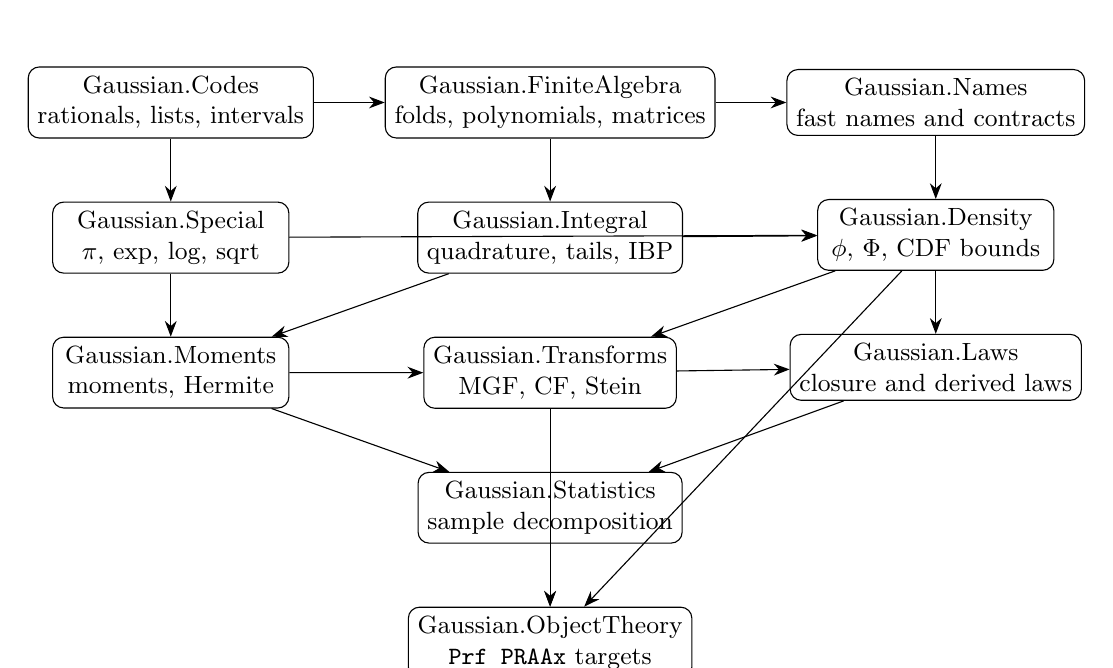
\begin{tikzpicture}[
  node distance=8mm and 9mm,
  box/.style={draw,rounded corners,align=center,minimum width=30mm,minimum height=8mm,font=\small},
  arr/.style={-{Stealth[length=2mm]}}
]
\node[box] (codes) {Gaussian.Codes\\rationals, lists, intervals};
\node[box, right=of codes] (finite) {Gaussian.FiniteAlgebra\\folds, polynomials, matrices};
\node[box, right=of finite] (names) {Gaussian.Names\\fast names and contracts};
\node[box, below=of codes] (special) {Gaussian.Special\\$\pi$, exp, log, sqrt};
\node[box, below=of finite] (integral) {Gaussian.Integral\\quadrature, tails, IBP};
\node[box, below=of names] (density) {Gaussian.Density\\$\phi$, $\Phi$, CDF bounds};
\node[box, below=of special] (moments) {Gaussian.Moments\\moments, Hermite};
\node[box, below=of integral] (trans) {Gaussian.Transforms\\MGF, CF, Stein};
\node[box, below=of density] (laws) {Gaussian.Laws\\closure and derived laws};
\node[box, below=of trans] (stats) {Gaussian.Statistics\\sample decomposition};
\node[box, below=of stats] (object) {Gaussian.ObjectTheory\\\code{Prf PRAAx} targets};
\draw[arr] (codes)--(finite);
\draw[arr] (finite)--(names);
\draw[arr] (codes)--(special);
\draw[arr] (finite)--(integral);
\draw[arr] (names)--(density);
\draw[arr] (special)--(density);
\draw[arr] (integral)--(density);
\draw[arr] (special)--(moments);
\draw[arr] (integral)--(moments);
\draw[arr] (density)--(trans);
\draw[arr] (moments)--(trans);
\draw[arr] (density)--(laws);
\draw[arr] (trans)--(laws);
\draw[arr] (laws)--(stats);
\draw[arr] (moments)--(stats);
\draw[arr] (stats)--(object);
\draw[arr] (trans)--(object);
\draw[arr] (density)--(object);
\end{tikzpicture}
\end{center}

\subsection{Layer 1: executable finite mathematics}

The first layer should compile independently of the embedded logic and should contain no analytic axioms.
\begin{enumerate}[label=\arabic*.]
  \item Define signed rationals, dyadics, outward intervals, list codes, and polynomial coefficient arrays, reusing repository types where convenient.
  \item Implement \code{atanPartial} and \code{piInterval}.
  \par Implement \code{sqrtInterval} and \code{expNegInterval}.
  \par Implement \code{cdfTaylorInterval}, following
  \path{code/gaussian_certificates.py}.
  \item Prove each interval constructor sound over Lean's integers/rationals.  These are ordinary metatheoretic proofs, not yet object-language derivations.
  \item Define \code{hermite : Nat -> Polynomial Int} and \code{normalMoment : Nat -> Nat}; prove the recurrences and coefficient identities.
  \item Define finite-law expectation, variance, product laws, and exact independence tables.  Reuse the central-limit packet's finite-law conventions when promoted into the repository.
\end{enumerate}
The executable layer provides trusted test vectors and lets later object formulas refer to concrete program syntax without manually transcribing large recursors.

\subsection{Layer 2: represented analysis contracts}

Define structures whose fields are data plus proofs, rather than declaring a typeclass instance for an unspecified classical function.  Suggested signatures are:
\begin{lstlisting}[language={}] 
structure FastName where
  eval : Nat -> Rat
  regular : forall p q, abs (eval p - eval q) <= dy p + dy q

structure BoundedFunName where
  eval : Rat -> Nat -> Rat
  modulus : Nat -> Nat
  bound : Nat -> Nat
  regular : ...

structure ImproperIntegralCert where
  cutoff : Nat -> Nat
  mesh : Nat -> Nat
  tail_ok : ...
  mesh_ok : ...
\end{lstlisting}
The actual types should match repository rational infrastructure.  Derivative, logarithm-apartness, matrix-positive-definiteness, and density-tail certificates are analogous.  The point is that no theorem receives a bare \code{Real -> Real} and then attempts to extract a modulus nonconstructively.

Ambient Lean can first prove that the certificate combinators are sound.  This establishes the mathematical dependency graph and catches missing hypotheses.  It is not yet the final \ipra{} result.

\subsection{Layer 3: primitive-recursive syntax}

For every executable producer and checker, construct the corresponding \code{PR k} term.  The order should be:
\begin{enumerate}[label=(\roman*)]
  \item integer/rational coding and interval Booleans;
  \item bounded folds, factorial, double factorial, powers, and coefficient lists;
  \item bisection and finite alternating sums;
  \item CDF and tail certificate checkers;
  \item Hermite and moment checkers;
  \item finite matrices, pairings, and sample-statistic checkers.
\end{enumerate}
Prove their defining equations in \code{Prf PRAAx}.  The central theorem for each program should have the form ``the graph formula is equivalent to equality with the \code{PTm} application.''  This permits rewriting inside larger object proofs.

\subsection{Layer 4: object arithmetic lemmas}

Develop the following checked derivations, using existing IPRADerivations wherever possible:
\begin{itemize}
  \item interval arithmetic soundness;
  \item alternating-sum bracketing;
  \item integer square-root bisection invariant;
  \item finite binomial, factorial, double-factorial, and Hermite coefficient identities;
  \item summation by parts and bounded Riemann refinement inequalities;
  \item matrix quadratic-form and Pythagorean identities;
  \item finite Jensen/log-sum-exp inequality needed for \cref{thm:expected-max}.
\end{itemize}
The repository's ring tool should dispatch many coefficient and sum-of-squares equalities after finite sums are normalized.

\subsection{Layer 5: target sentences}

The file \code{lean/ObjectLanguageTargets.lean} sketches the target families.  Representative mathematical forms are:
\begin{align*}
 \operatorname{CDFBound}(x,p,L,U)
 &:\equiv L\le\Phi_p(x)\wedge\Phi_p(x)\le U\wedge U-L\le2^{-p},\\
 \operatorname{Moment}(n,p,m)
 &:\equiv |I_{n,p}-m|\le2^{-p},\\
 \operatorname{Mills}(x,p)
 &:\equiv \frac{x}{1+x^2}\phi_p(x)<Q_p(x)<\frac{\phi_p(x)}x
       \quad\text{up to }2^{-p},\\
 \operatorname{HermiteDeriv}(n,x,p)
 &:\equiv |D^n\phi_p(x)-(-1)^n\He_n(x)\phi_p(x)|\le2^{-p}.
\end{align*}
Here every apparent analytic symbol is an abbreviation for a finite evaluator and certificate code.  The theorem statement exposed to \code{Prf} contains only natural-number variables, equalities, and order predicates.

\subsection{Layer 6: ordinary-to-native transport}

After constructing
\[
 h_A : []\vdash[\code{PRAAx}]A,
\]
apply the existing bridge to obtain the native derivation.  The exact invocation should be taken from the current signature of \code{pra\_iff\_native}; no new semantic axiom is required.  Keep both endpoints in the module:
\begin{itemize}
  \item the ordinary theorem, because its formulas are readable and compose with IPRADerivations;
  \item the transported native theorem, because it demonstrates compatibility with the smallest concise presentation.
\end{itemize}

\subsection{Recommended completion order}

A realistic sequence that yields useful checked milestones is:
\begin{enumerate}
  \item Hermite coefficient identities and exact moment recurrence.
  \item Exact affine, sum-of-squares, and MLE identities.
  \item Machin $\pi$, square-root, and exponential interval producers.
  \item Certified CDF values at integer arguments and the $68$--$95$--$99.7$ theorem.
  \item Mills inequalities and the quantile bisection checker.
  \item General represented normalization and integration by parts.
  \item MGF/CF, convolution closure, and multivariate projections.
  \item Entropy/KL/Fisher formulas.
  \item Sample decomposition, chi-square, $t$, and $F$.
  \item General maximum entropy and effective transform uniqueness.
\end{enumerate}
The first four milestones are largely bounded arithmetic and would already turn a substantial portion of this packet into kernel-checked object mathematics.

\subsection{Axiom and status audit}

The completed development should run three audits:
\begin{enumerate}[label=(\roman*)]
  \item reject \code{sorry}, \code{admit}, and newly introduced axioms;
  \item print the axioms of every exported ambient theorem;
  \item ensure every headline object theorem literally has type \code{Prf PRAAx [] $\varphi$} or its notation equivalent.
\end{enumerate}
The present archive passes its Python validation and PDF build, but because Lean was unavailable it makes no statement about Lean compilation.  This limitation is repeated in the README and manifest so that an outline cannot be mistaken for a formal proof.

\section{Statement-by-statement coverage}\label{sec:coverage}

This section summarizes the main claims appearing on the inspected Wikipedia and MathWorld pages.  The separate \code{THEOREM\_LEDGER.md} gives a more granular list, corrections, and cross-references.

\small
\begin{longtable}{@{}>{\raggedright\arraybackslash}p{0.34\textwidth} c >{\raggedright\arraybackslash}p{0.46\textwidth}@{}}
\toprule
Source claim family & Status & Result in this package\\
\midrule
\endfirsthead
\toprule
Source claim family & Status & Result in this package\\
\midrule
\endhead
Density and parameterization by $\mu,\sigma^2$ & P & Definition \eqref{eq:normal-density}; effective scale apartness is explicit.\\
Standard normal and standardization & P & \Cref{thm:normalization-standardization}.\\
Normalization of the density & P/R & Gamma substitution and $\Gamma(1/2)=\sqrt\pi$, \eqref{eq:gaussian-normalization}.\\
CDF and error function & P & \Cref{cor:cdf-erf}.\\
Quantile function & E & Primitive-recursive interval-valued inverse, \cref{thm:quantile}; no real trichotomy.\\
Support is all real numbers & E & Every rational interval gets a computable positive lower bound, \cref{cor:support}.\\
Mean, median, mode & P & All equal $\mu$, \cref{thm:centers}.\\
Variance and standard deviation & P & $\sigma^2$ and $\sigma$, \cref{thm:centers}.\\
Mean absolute deviation & P & $\sigma\sqrt{2/\pi}$, \cref{cor:shape-statistics}.\\
Median absolute deviation & P & $\sigma\Phi^{-1}(3/4)$, \cref{cor:shape-statistics}.\\
Skewness and kurtosis & P & $0$, $3$, and zero excess.\\
Density peak and inflection points & P & Peak at $\mu$, inflections at $\mu\pm\sigma$, \cref{prop:shape}.\\
Symmetry & P & \eqref{eq:cdf-symmetry} and even density.\\
Log-concavity & P & Constant negative second derivative of log density.\\
Density/CDF ODEs & P & \Cref{prop:gaussian-odes}.\\
Taylor series for $\Phi$ & P & Finite formula and explicit remainder, \cref{thm:cdf-taylor}.\\
Density-factor series for $\Phi$ & C/P & It is globally convergent, not merely asymptotic; \cref{thm:cdf-density-series}.\\
Tail estimates & P & Mills inequalities and arbitrary finite expansion, \cref{thm:mills,thm:mills-expansion}.\\
$68$--$95$--$99.7$ rule & P & Exact-rational certified intervals for $n=1,\dots,6$, \cref{cor:coverage}.\\
Newton computation of quantiles & E & Safeguarded Newton with explicit entry and quadratic-error bounds, \cref{alg:newton}.\\
Raw and central moments & P & \Cref{thm:moment-recurrence,cor:raw-moments}.\\
Absolute moments & P/R & Gamma formula \eqref{eq:absolute-moment}.\\
Hermite derivative identities & P & \Cref{thm:hermite-derivatives}.\\
Hermite orthogonality/generating function & P & \Cref{cor:hermite-orthogonality,cor:hermite-generating}.\\
Conditional mean on an interval & P & \eqref{eq:trunc-mean}; conditional variance also proved.\\
Fourier transform & P/R & \Cref{thm:transforms,cor:self-fourier}; quantitative route reused from zeta packet.\\
MGF and characteristic function & P & \eqref{eq:mgf}--\eqref{eq:cf}.\\
Cumulants & P & First two nonzero; all higher vanish, \cref{cor:cumulants}.\\
Stein operator and characterization & E & \Cref{thm:stein,thm:stein-characterization}.\\
Differential entropy & P & \eqref{eq:entropy}.\\
Maximum entropy & E & Effective-density form with explicit integrability, \cref{thm:max-entropy}.\\
KL divergence & P & Closed formula \eqref{eq:kl-normal} and constructive positivity.\\
Hellinger distance & P & \eqref{eq:hellinger}.\\
Fisher information & P & Both common parameterizations, \cref{thm:fisher}.\\
Expected maximum bound & P & No independence needed, \cref{thm:expected-max}.\\
Affine transformations & P & \Cref{thm:normalization-standardization}.\\
Sums and convolution closure & P & \Cref{thm:linear-combination}.\\
Stability & P & \Cref{cor:stability}.\\
Infinite divisibility & P & One finite convolution identity for every $n$.\\
Normalized product of densities & P & Precision-weighted pooling, \cref{prop:product-densities}.\\
Multivariate normal/projections & E/P & Positive-definite effective matrices, \cref{thm:multivariate-normal,cor:projections}.\\
Joint normal plus zero covariance implies independence & P & \Cref{thm:joint-normal-independence}.\\
Independence of sum and difference & P & \Cref{cor:sum-difference}.\\
Conditional bivariate normal & E/P & Nondegenerate case with an explicit $1-\rho^2$ bound, \cref{thm:bivariate-conditional}.\\
Absolute/folded/half-normal law & P & \Cref{thm:folded-normal}.\\
Square gives chi-square & P & Central and noncentral one-dimensional versions, \cref{thm:normal-square}.\\
Sum of squares/chi law/Rayleigh/Maxwell & P & \Cref{thm:chi-square,cor:chi-radius}.\\
Ratio of centered normals is Cauchy & C/P & Centering is essential; \cref{thm:normal-ratio}.\\
Product of centered normals & P & Characteristic function and $K_0$ density, \cref{thm:product-normal}.\\
Exponentiation gives lognormal & P & Density and moments, \cref{thm:lognormal}.\\
Sample mean distribution & P & Exact for Gaussian samples, \eqref{eq:mean-law}.\\
Sample variance and independence & P & \Cref{thm:sample-decomposition}.\\
MLE for mean and variance & C/P & Formula plus correction for identical data, \cref{thm:mle}.\\
Bias/unbiased variance and variances & P & \Cref{cor:sample-variance-moments}.\\
Student $t$ and Fisher $F$ laws & P/R & Gamma/beta change-of-variable proofs, \cref{thm:student,thm:f-distribution}.\\
Confidence pivots & E/P & Effective quantile versions, \cref{cor:confidence}.\\
Inverse-CDF simulation & E/P & Finite-bit implementation with boundary error, \cref{thm:inverse-transform}.\\
Box--Muller simulation & E/P & Truncated finite implementation and Jacobian proof, \cref{thm:box-muller}.\\
Zero-variance degeneration & C/P & Effective weak convergence; CDF convergence excludes the jump, \cref{thm:zero-variance}.\\
Central limit theorem and Berry--Esseen & R & Existing ProveIt packet, \cref{thm:clt-reuse}.\\
Exact normality of arbitrary averages & C & False in general; asymptotic quantitative statement in \cref{cor:sample-mean-clt}.\\
Marcinkiewicz polynomial-cumulant characterization & D & Forward Gaussian cumulants and analytic quadratic-MGF criterion proved; full converse omitted.\\
Cramer decomposition theorem & D & Requires a separate factorization theorem for entire characteristic functions.\\
Kac--Bernstein theorem & D & Requires a separate functional-equation argument.\\
Geary characterization & D & Forward mean/variance independence proved; converse omitted.\\
Information-geometric constant curvature & D & Fisher metric is computed; global curvature development is outside this packet.\\
Full exact variance formulas for high sample skewness/kurtosis statistics & D & Reducible to finite Wick enumeration, but the long combinatorial simplifications are not reconstructed.\\
Claims about non-elementarity of the CDF & D & This is a differential-algebra theorem, not needed for effective evaluation.\\
Historical, empirical, and application claims & D & Not mathematical identities in the requested proof-theoretic sense.\\
\bottomrule
\end{longtable}
\normalsize

\subsection{Assessment}

The elementary normal theory is unusually well suited to \ipra.  Its essential proofs are finite completion of squares, integration by parts with explicit Gaussian tails, polynomial recurrences, and finite-dimensional linear algebra.  The genuine boundary lies not at transcendental constants or improper integrals---those have direct primitive-recursive names---but at deep converse characterization theorems and at statements whose classical wording suppresses effectivity.  The packet proves the forward Gaussian mathematics and exposes those boundaries rather than filling them with semantic assumptions.


\appendix
\section{Finite lemmas used repeatedly}\label{app:finite-lemmas}

This appendix collects the elementary identities that carry most of the arithmetization.  Each is a theorem of finite algebra or bounded induction.

\begin{lemma}[Product telescoping]\label{lem:product-telescope}
For any commutative ring and finite lists $a_0,\dots,a_{n-1}$ and $b_0,\dots,b_{n-1}$,
\begin{equation}\label{eq:product-telescope}
 \prod_{j<n}a_j-\prod_{j<n}b_j
 =\sum_{k<n}(a_k-b_k)
   \left(\prod_{j<k}a_j\right)
   \left(\prod_{k<j<n}b_j\right).
\end{equation}
Consequently, if $|a_j|,|b_j|\le M$, then
\[
 \left|\prod a_j-\prod b_j\right|
 \le M^{n-1}\sum_j|a_j-b_j|.
\]
\end{lemma}

\begin{proof}
Induct on $n$.  The successor step adds and subtracts
$a_n\prod_{j<n}b_j$, then applies the induction hypothesis.  The inequality is the finite triangle inequality.  This lemma propagates interval errors through exponentiation, likelihood products, and characteristic-function products.
\end{proof}

\begin{lemma}[Finite summation by parts]\label{lem:summation-parts}
For finite sequences $u_j,v_j$ and forward differences
$\Delta v_j=v_{j+1}-v_j$,
\begin{equation}\label{eq:summation-parts}
 \sum_{j=0}^{n-1}u_j\Delta v_j
 =u_{n-1}v_n-u_0v_0-\sum_{j=0}^{n-2}v_{j+1}(u_{j+1}-u_j).
\end{equation}
\end{lemma}

\begin{proof}
Expand both sums and cancel adjacent terms.  Bounded induction on $n$ formalizes the cancellation.  Finite integration by parts is obtained by taking $u_j$ and $v_j$ to be sampled function values and controlling the difference-quotient residuals.
\end{proof}

\begin{lemma}[Alternating enclosure]\label{lem:alternating}
Let $a_0\ge a_1\ge\cdots\ge a_N\ge0$.  Then every partial alternating sum after $N$ lies between the last even and odd partial sums.  If a supplied tail majorant proves $a_N\to0$ effectively, the value of the represented series lies between $S_N$ and $S_N+(-1)^Na_N$.
\end{lemma}

\begin{proof}
Pair neighboring terms: $a_{2j}-a_{2j+1}\ge0$.  Even partial sums decrease and odd partial sums increase, while each even sum is above the following odd sum.  The claim for a finite later cutoff is quantifier-free induction.  The tail modulus identifies the common represented limit.
\end{proof}

\begin{lemma}[Bisection without real trichotomy]\label{lem:robust-bisection}
Let $F$ be increasing on $[a,b]$ with an effective lower slope $m>0$:
$F(y)-F(x)\ge m(y-x)$ for $x\le y$.  Suppose $F(c)$ can be enclosed within radius $\varepsilon$ at every rational $c$.  Given $p$, midpoint bisection may use the following three-way bounded rule:
\begin{enumerate}[label=(\roman*)]
 \item if the enclosure is below $p$, keep the right half;
 \item if it is above $p$, keep the left half;
 \item if it contains $p$, return $[c-\varepsilon/m,c+\varepsilon/m]$.
\end{enumerate}
The returned interval contains every solution of $F(x)=p$ and has a primitive-recursive width bound.
\end{lemma}

\begin{proof}
Only rational interval comparisons are used.  In the third case,
$|F(c)-p|\le\varepsilon$, while the lower slope gives
$m|c-q|\le|F(c)-F(q)|$.  Ordinary bisection handles the other cases.  This is the constructive pattern used for Gaussian quantiles and all continuous positive-density pivots.
\end{proof}

\begin{lemma}[Completion of squares]\label{lem:complete-square}
For $\sigma>0$,
\begin{align*}
 tx-\frac{(x-\mu)^2}{2\sigma^2}
 &=-\frac{(x-\mu-\sigma^2t)^2}{2\sigma^2}
   +\mu t+\frac12\sigma^2t^2,\\
 \frac{(x-\mu_0)^2}{4\sigma_0^2}
 +\frac{(x-\mu_1)^2}{4\sigma_1^2}
 &=A(x-m)^2+C,
\end{align*}
where $A,m,C$ are the rational expressions used in the Hellinger calculation.  Every Gaussian MGF, product-of-densities, conditional, and Hellinger formula is obtained by one such ring identity followed by normalization.
\end{lemma}

\begin{proof}
Multiply through by the positive common denominator and normalize both sides as polynomials in $x$.  Prove equality coefficientwise using the repository ring tactic or its object-language certificate.
\end{proof}

\begin{lemma}[Gaussian anti-concentration on bounded intervals]\label{lem:anti-concentration}
For every rational interval $I=[a,b]$,
\[
 0<\int_a^b\phi(x)\dd x
 \le (b-a)\phi(0),
\]
and if $|a|,|b|\le B$,
\[
 \int_a^b\phi(x)\dd x
 \ge(b-a)\phi(B).
\]
\end{lemma}

\begin{proof}
On $[-B,B]$, monotonicity in $|x|$ gives
$\phi(B)\le\phi(x)\le\phi(0)$.  Multiply by the interval length using finite lower and upper Riemann sums.  This lemma supplies positive denominators for truncated means and lower derivatives for quantile inversion.
\end{proof}

\begin{lemma}[Finite Gaussian moment tail]\label{lem:moment-tail}
For every externally fixed $n$ there is a primitive-recursive $T(n,p)$ such that
\[
 \int_{|x|>T(n,p)}|x|^n\phi(x)\dd x\le2^{-p}.
\]
The same cutoff can make all boundary terms $|x|^j\phi(x)$, $j\le n+1$, at most $2^{-p}$.
\end{lemma}

\begin{proof}
Use \eqref{eq:poly-gaussian-tail}, absorb the fixed normalizing constant by the rational bound $(2\pi)^{-1/2}<1$, and find $T$ by bounded search until the explicit exponential majorant is below $2^{-p}$.  Exponential evaluation itself has the finite enclosure of \eqref{eq:exp-alt}.
\end{proof}

\begin{lemma}[Finite change of variables]\label{lem:finite-cov}
Let $y=g(x)$ be monotone on a compact rational interval, with effective derivative and inverse contracts and a derivative apartness witness.  Then the transformed tagged sums differ by at most an explicit function of the source mesh, evaluator errors, and the moduli of $f,g,g^{-1}$ from
\[
 \int f(g(x))g'(x)\dd x=\int f(y)\dd y.
\]
For the affine, square, exponential, and polar substitutions in this manuscript, this error function is primitive recursive.
\end{lemma}

\begin{proof}
Map every source cell to a target interval.  The exact mean-value identity is replaced by the derivative contract, which controls the target cell length.  Compare the source and target sample values through the supplied moduli, sum the local errors, and use the mesh bound.  Improper endpoints are removed separately by their explicit tails.  This is the finite proof behind every displayed change of variables.
\end{proof}

\section{Executable certificate summary}\label{app:certificates}

The command
\begin{lstlisting}
python3 code/gaussian_certificates.py \
  --output evidence/validation.json \
  --summary evidence/validation.txt
\end{lstlisting}
performs 96 checks.  All proof-relevant numerical operations use Python integers and \code{fractions.Fraction}.  The script may also print high-precision \code{mpmath} diagnostics, but these are explicitly labeled non-authoritative and are never used to decide a check.

The exact-rational checks include:
\begin{itemize}
  \item a Machin-series interval for $\pi$ and a dyadic interval for $(2\pi)^{-1/2}$;
  \item six CDF/coverage certificates from the alternating integrated exponential series;
  \item both Mills inequalities at $x=1,\dots,6$;
  \item the standard moment recurrence and exact values through order $20$;
  \item the general raw-moment recurrence for a nontrivial rational $(\mu,\sigma^2)$ test instance;
  \item Gaussian derivative/Hermite identities through order $14$;
  \item the Hermite three-term and derivative recurrences through order $14$;
  \item exact finite-law mean/variance and the least-squares center identity;
  \item symbolic regression checks for score functions, KL and Hellinger self-values, and the Box--Muller polar Jacobian.
\end{itemize}

The recorded central coverage displays are:
\begin{lstlisting}
All checks passed: True
Checks: 96 / 96
n=1  0.68268949213708589717...
n=2  0.95449973610364158560...
n=3  0.99730020393673981095...
n=4  0.99993665751633376016...
n=5  0.99999942669685624161...
n=6  0.99999999802682470992...
\end{lstlisting}
The full JSON records outward rational endpoints, not only decimals.  The script rounds intermediate transcendental enclosures outward to fixed dyadic grids, so its certificate sizes remain manageable and every subsequent interval operation remains exact.

These computations serve three purposes: they test the formulas, provide finite examples for the proposed Lean implementation, and demonstrate that the precision schedules are genuinely primitive recursive.  They do not replace the universal proofs in the manuscript or the future object-language derivations.


\begin{thebibliography}{99}
\bibitem{WikipediaNormal}
Wikipedia contributors, ``Normal distribution,'' \emph{Wikipedia, The Free Encyclopedia}, snapshot inspected 16 November 2026.\\
\url{https://en.wikipedia.org/wiki/Normal_distribution}

\bibitem{MathWorldNormal}
E. W. Weisstein, ``Normal Distribution,'' \emph{MathWorld---A Wolfram Web Resource}, snapshot inspected 16 November 2026.\\
\url{https://mathworld.wolfram.com/NormalDistribution.html}

\bibitem{ProveIt}
V. Reshetnikov, \emph{ProveIt}, repository snapshot \commitsha.\\
\url{https://github.com/VladimirReshetnikov/ProveIt}

\bibitem{ConciseIPRA}
V. Reshetnikov et al., ``Concise presentations of intuitionistic primitive recursive arithmetic,'' in \path{Logic/PrimitiveRecursiveArithmetic/ConciseIPRA} of \cite{ProveIt}.

\bibitem{CLTIPRA}
``Constructive central limit theorems in iPRA,'' in \path{Logic/PrimitiveRecursiveArithmetic/docs/proofs/probability/central_limit_ipra_2026-11-15} of \cite{ProveIt}.

\bibitem{CalculusIPRA}
``The fundamental theorem of calculus and the Euler--Maclaurin formula in iPRA,'' in \path{Logic/PrimitiveRecursiveArithmetic/docs/proofs/analysis/calculus_ipra} of \cite{ProveIt}.

\bibitem{GammaIPRA}
``Gamma in intuitionistic primitive recursive arithmetic,'' in \path{Logic/PrimitiveRecursiveArithmetic/docs/proofs/analysis/gamma_ipra} of \cite{ProveIt}.

\bibitem{TaylorIPRA}
``Taylor's theorem and Cauchy's integral formula in iPRA,'' in \path{Logic/PrimitiveRecursiveArithmetic/docs/proofs/analysis/taylor_cauchy_ipra} of \cite{ProveIt}.

\bibitem{ZetaIPRA}
``Constructive zeta theory,'' especially its certified Gaussian Fourier transform, in \path{Logic/PrimitiveRecursiveArithmetic/docs/proofs/analytic-number-theory/zeta_ipra} of \cite{ProveIt}.

\bibitem{Feller}
W. Feller, \emph{An Introduction to Probability Theory and Its Applications}, vol. 1, Wiley.

\bibitem{JohnsonKotz}
N. L. Johnson, S. Kotz, and N. Balakrishnan, \emph{Continuous Univariate Distributions}, vol. 1, Wiley.
\end{thebibliography}

\end{document}
